\documentclass{../preparationclass}

\newcommand{\whichprep}{Ex}
\newcommand{\vornamea}{Umut}
\newcommand{\vornameb}{-}
\newcommand{\nachnamea}{Elicabuk}
\newcommand{\nachnameb}{-}

\begin{document}

	\begin{titlepage}

	\newcommand{\Hrule}{\rule{\linewidth}{0.5mm}}
	\center
	%title
	\Hrule\\[0.4cm]
	{\huge\bfseries \whichprep -Vorbereitung}\\[0.2cm]
	\Hrule\\[1.5cm]

	%are we human, or are we dancer?
	\begin{minipage}{0.4\textwidth}
		\begin{flushleft}
			\large
			\textit{Autor}\\
			\vornamea\ \textsc{\nachnamea}\\
		\end{flushleft}
	\end{minipage}
	~
	\begin{minipage}{0.4\textwidth}
		\begin{flushright}
			\large
			\textit{Autor}\\
			\vornameb\ \textsc{\nachnameb}\\
		\end{flushright}
	\end{minipage}\par
	\vspace{1cm}

	\large
	\textit{Datum}\\
	\today

\end{titlepage}

	%% Custom commands used throughout the summaries
%% @author Umut Elicabuk
%% @date 11.05.2018
%% ---------------------------------------------

\newcommand{\diff}[2][]{\ensuremath{\frac{\text{d} #1}{\text{d} #2}}}						% for derivatives, first argument is optional and will be omitted if not specified
\newcommand{\ddiff}[3][]{\ensuremath{\frac{\text{d}^2 #1}{\text{d} #2 \text{d} #3}}}
\newcommand{\mvec}[1]{\boldsymbol{#1}}																					% for vectors, conventionally bold letters
\newcommand{\el}{\ensuremath{\text{e}^-}}
\newcommand{\pos}{\ensuremath{\text{e}^+}}

	\tableofcontents
	\clearpage
	\setcounter{page}{1}

	\chapter{Einführung}
Hallöle.
Auf den folgenden Seiten findet ihr meine Zusammenfassungen zur mündlichen Prüfung in \whichprep.
Musste das sowieso texen, um es abends nochmal zu wiederholen, also habt kein schlechtes Gewissen beim Durchstöbern.
Viel Erfolg bei eurer Prüfung, ihr schafft das schon, ENDSPURT!!!

Euer Umut
Dichter, Denker, Playboy

	\chapter{Geometrische Gestalt der Kerne}

\section{Mandelstam-Variablen}
Betrachten die Reaktion zweier Teilchen mit den 4-Impulsen $p_1$ und $p_2$. Die auslaufenden Teilchen sollen die 4-Impulse $p_3$ und $p_4$ haben.
Dann kann man die sogen. \textbf{Mandelstam-Variablen}
\begin{alignat*}{5}
	s &= \left(p_1 + p_2 \right)^2 &&= \left(p_3 + p_4 \right)^2 &&\stackrel{\text{LS}}{=} 2m_2E_1 &&\stackrel{CMS}{=}4E^2\\
	t &= \left(p_1 - p_3 \right)^2 &&= \left(p_4 - p_2 \right)^2 &&\stackrel{\text{LS}}{=} 2m_2(E_3-E_1) &&\stackrel{CMS}{=} \frac{s}{2}(\cos\theta-1)\\
	u &= \left(p_1 - p_4 \right)^2 &&= \left(p_3 - p_2 \right)^2 &&\stackrel{\text{LS}}{=} -2m_2E_3 &&\stackrel{CMS}{=}-\frac{s}{2}(\cos\theta+1).
\end{alignat*}
$s$ ist dabei das Quadrat der Schwerpunktsenergie des Systems und $u$ entspricht dem Quadrat des 4-Impulsübertrags einer gewöhnlichen Streuung.
Die Mandelstam-Variablen sind Lorentzskalare.

\section{Die Rapidität}
Die Rapidität ist ein Maß für Geschwindigkeiten in der Relativistik.
Sie ist definiert als
\begin{equation*}
	y = \frac{1}{2}\log\left(\frac{E+cp}{E-cp}\right)\quad \text{bzw. als}\quad y_L=\frac{1}{2}\log\left(\frac{E+cp_\text{z}}{E-cp_\text{z}}\right)
\end{equation*}
in der Teilchenphysik.
Anders als die Geschwindigkeit $v$ eines Teilchens ist die Rapidität nicht auf das Intervall $[-c,\ +c]$ beschränkt, sondern ist unbeschränkt.
Sie gibt ein intuitiveres Gefühl dafür, welche Geschwindigkeit ein Teilchen hätte, würde es keine relativistischen Effekte erfahren.
Außerdem sind Differenzen von zwei Rapiditäten invariant unter Lorentzboosts entlang der Strahlachse und man kann Rapiditäten einfach addieren, anders als Geschwindigkeiten ($\rightarrow$ rel. Geschwindigkeitsaddition).
Aufgrund dieser Invarianz unter Lorentzboosts wird die Angabe von $y$ gegenüber dem Polarwinkel $\theta$ bevorzugt.

Für den Fall $E\gg m$ geht die Rapidität über in die sogen. \textbf{Pseudorapidität}
\begin{equation*}
	\eta = -\log\left(\tan\left(\frac{\theta}{2}\right)\right).
\end{equation*}

Der diferenzielle Wirkungsquerschnitt $\nicefrac{\text{d}\sigma}{\text{d}y}$ ist forminvariant unter Lorentzboosts entlang der Strahlachse.
Das gleiche gilt in guter Näherung auch für $\nicefrac{\text{d}\sigma}{\text{d}\eta}$, allerdings ist $\eta$ einfacher zu messen, da man nur die Flugrichtung des Teilchens durch den Detektor bestimmen muss.

\section{Elastische Streuung punktförmiger Teilchen}
Streuexperimente dienen dazu, Mikroskopie über das sichtbare hinaus zu betreiben und so Erkenntnisse über die Struktur der Materie zu gewinnen.
Man unterscheidet dabei zwischen \textbf{elastischer} ($\sum E_{\text{kin,}i} = \sum E_{\text{kin,}f}$) und \textbf{inelastischer Streuung} ($\sum E_{\text{kin,}i} \neq \sum E_{\text{kin,}f}$, z.B. durch Anregung eines Atoms durch Teil der kinetischen Energie).

Der Wirkungsquerschnitt ist die wichtigste Größe bei solchen Experimenten und ist ein Maß dafür, wie wahrscheinlich eine Wechselwirkung zwischen dem Projektil und dem Target ist.
Experimentell gilt
\begin{equation*}
	\sigma = \frac{N_\text{obs}-N_\text{bg}}{\mathcal{L}\cdot\varepsilon\cdot A}\cdot\frac{1}{T},
\end{equation*}
mit der weiteren wichtigen Detektorkenngröße, der \textbf{Luminosität} $\mathcal{L}$, die die Anzahl der Teilchenbegegnungen pro Zeit und Fläche beschreibt.
Für Effizienz $\varepsilon$ und Akzeptanz $A$, siehe \url{https://www.spektrum.de/lexikon/physik/nachweisempfindlichkeit/10087}.

\subsection{Rutherford-Wirkungsquerschnitt}
Der Rutherfordsche Wirkungsquerschnitt gibt den theoretischen Wirkungsquerschnitt unter Vernachlässigung von Spins und Targetrückstoß an
\begin{equation}\label{eq:ruth_sigma}
	\left(\diff[\sigma]{\Omega}\right)_\text{Ruth} = \left(\frac{zZe^2}{4\pi\epsilon_0\cdot 4E_\text{kin}}\right)^2\cdot\frac{1}{\sin^4\frac{\theta}{2}}.
\end{equation}
Problematisch erscheint hierbei zunächst, dass der Wirkungsquerschnitt für $\theta\rightarrow 0$ divergiert.
Allerdings gehören kleine Streuwinkel zu großen Stoßparametern weit entfernt vom Kern, wo die Elektronen bereits das Coulombfeld des Kernes abschirmen und somit die Formel für den Wirkungsquerschnitt nicht mehr anwendbar ist.

Definiert man den Impulsübertrag
\begin{equation*}
	\mvec{q} = \mvec{p}-\mvec{p'},
\end{equation*}
so lässt sich \autoref{eq:ruth_sigma} auch schreiben als
\begin{equation*}
	\left(\diff[\sigma]{\Omega}\right)_\text{Ruth} = \frac{4zZ\alpha^2(\hbar c)^2 E'^2}{|\mvec{q}c|^4}.
\end{equation*}
Durch die $\nicefrac{1}{q^4}$-Abhängigkeit ist es schwer, Prozesse mit hohem Impulsübertrag zu messen, da ein Fehler auf $\mvec{q}$ sich erheblich auf die Ergebnisse auswirkt.

Beachtet man, dass für kleine Massen $E\approx pc$ gilt, folgt daraus der \textbf{relativistische Rutherford-Wirkungsquerschnitt}
\begin{equation*}
	\left(\diff[\sigma]{\Omega}\right)_\text{Ruth} = \left(\frac{zZ\alpha\hbar c}{4mc^2(\gamma-1)}\right)^2\cdot\left(\frac{4p_1p_3}{q^2}\right)^2.
\end{equation*}

\subsection{Mott-Wirkungsquerschnitt}
Ist nun der Spin des Projektiles $\neq 0$, ergibt sich daraus der \textbf{Mott-Wirkungsquerschnitt}
\begin{equation*}
	\left(\diff[\sigma]{\Omega}\right)_\text{Mott} = \left(\diff[\sigma]{\Omega}\right)_\text{Ruth}\cdot\underbrace{\frac{E_\text{f}}{E}}_\text{Targetrückstoß}\cdot\underbrace{\left(1-\beta^2\sin^2\frac{\theta}{2}\right)}_\text{Spin d. Projektils}.
\end{equation*}
Für $\beta\rightarrow 1$ geht der Wirkungsquerschnitt über in
\begin{equation*}
	\left(\diff[\sigma]{\Omega}\right)_\text{Mott}= \rightarrow\left(\diff[\sigma]{\Omega}\right)_\text{Ruth}\cdot\frac{E_\text{f}}{E}\cdot\cos^2\frac{\theta}{2}.
\end{equation*}
Dabei sieht man, dass für $\beta\rightarrow 1$ ein Streuwinkel von 180° nicht möglich ist.
Dies folgt aus der Helizitätserhaltung: Bei einer Rückstreuung müsste auch der Spin flippen, damit die Projektion des Spins auf die Flugbahn (Helizität) erhalten bleibt. Dies ist jedoch an einem spinlosen Target aufgrund der Drehimpulserhaltung nicht möglich.

\subsection{Dirac-Wirkungsquerschnitt}
Bei der \textbf{Dirac-Streuung} haben nun beide Streupartner einen Spin.
Der Wirkungsquerschnitt wird dementsprechend modifiziert
\begin{equation*}
	\left(\diff[\sigma]{\Omega}\right)_\text{Dirac} = \left(\diff[\sigma]{\Omega}\right)_\text{Mott}\cdot\left(1+2\tau\tan^2\frac{\theta}{2}\right),
\end{equation*}
wobei $\tau = \frac{Q^2}{4M^2c^2}$.
Damit kann allerdings keine Streuung z.B. an realen Protonen beschrieben werden, da hier angenommen wird, dass das \textbf{punktförmige} ''Dirac-Proton'' ein herkömmliches magnetisches Moment von $\mu=\frac{e}{2m}$ besitzt.

\section{Elastische Streuung ausgedehnter Teilchen}

\begin{figure}
	\centering
	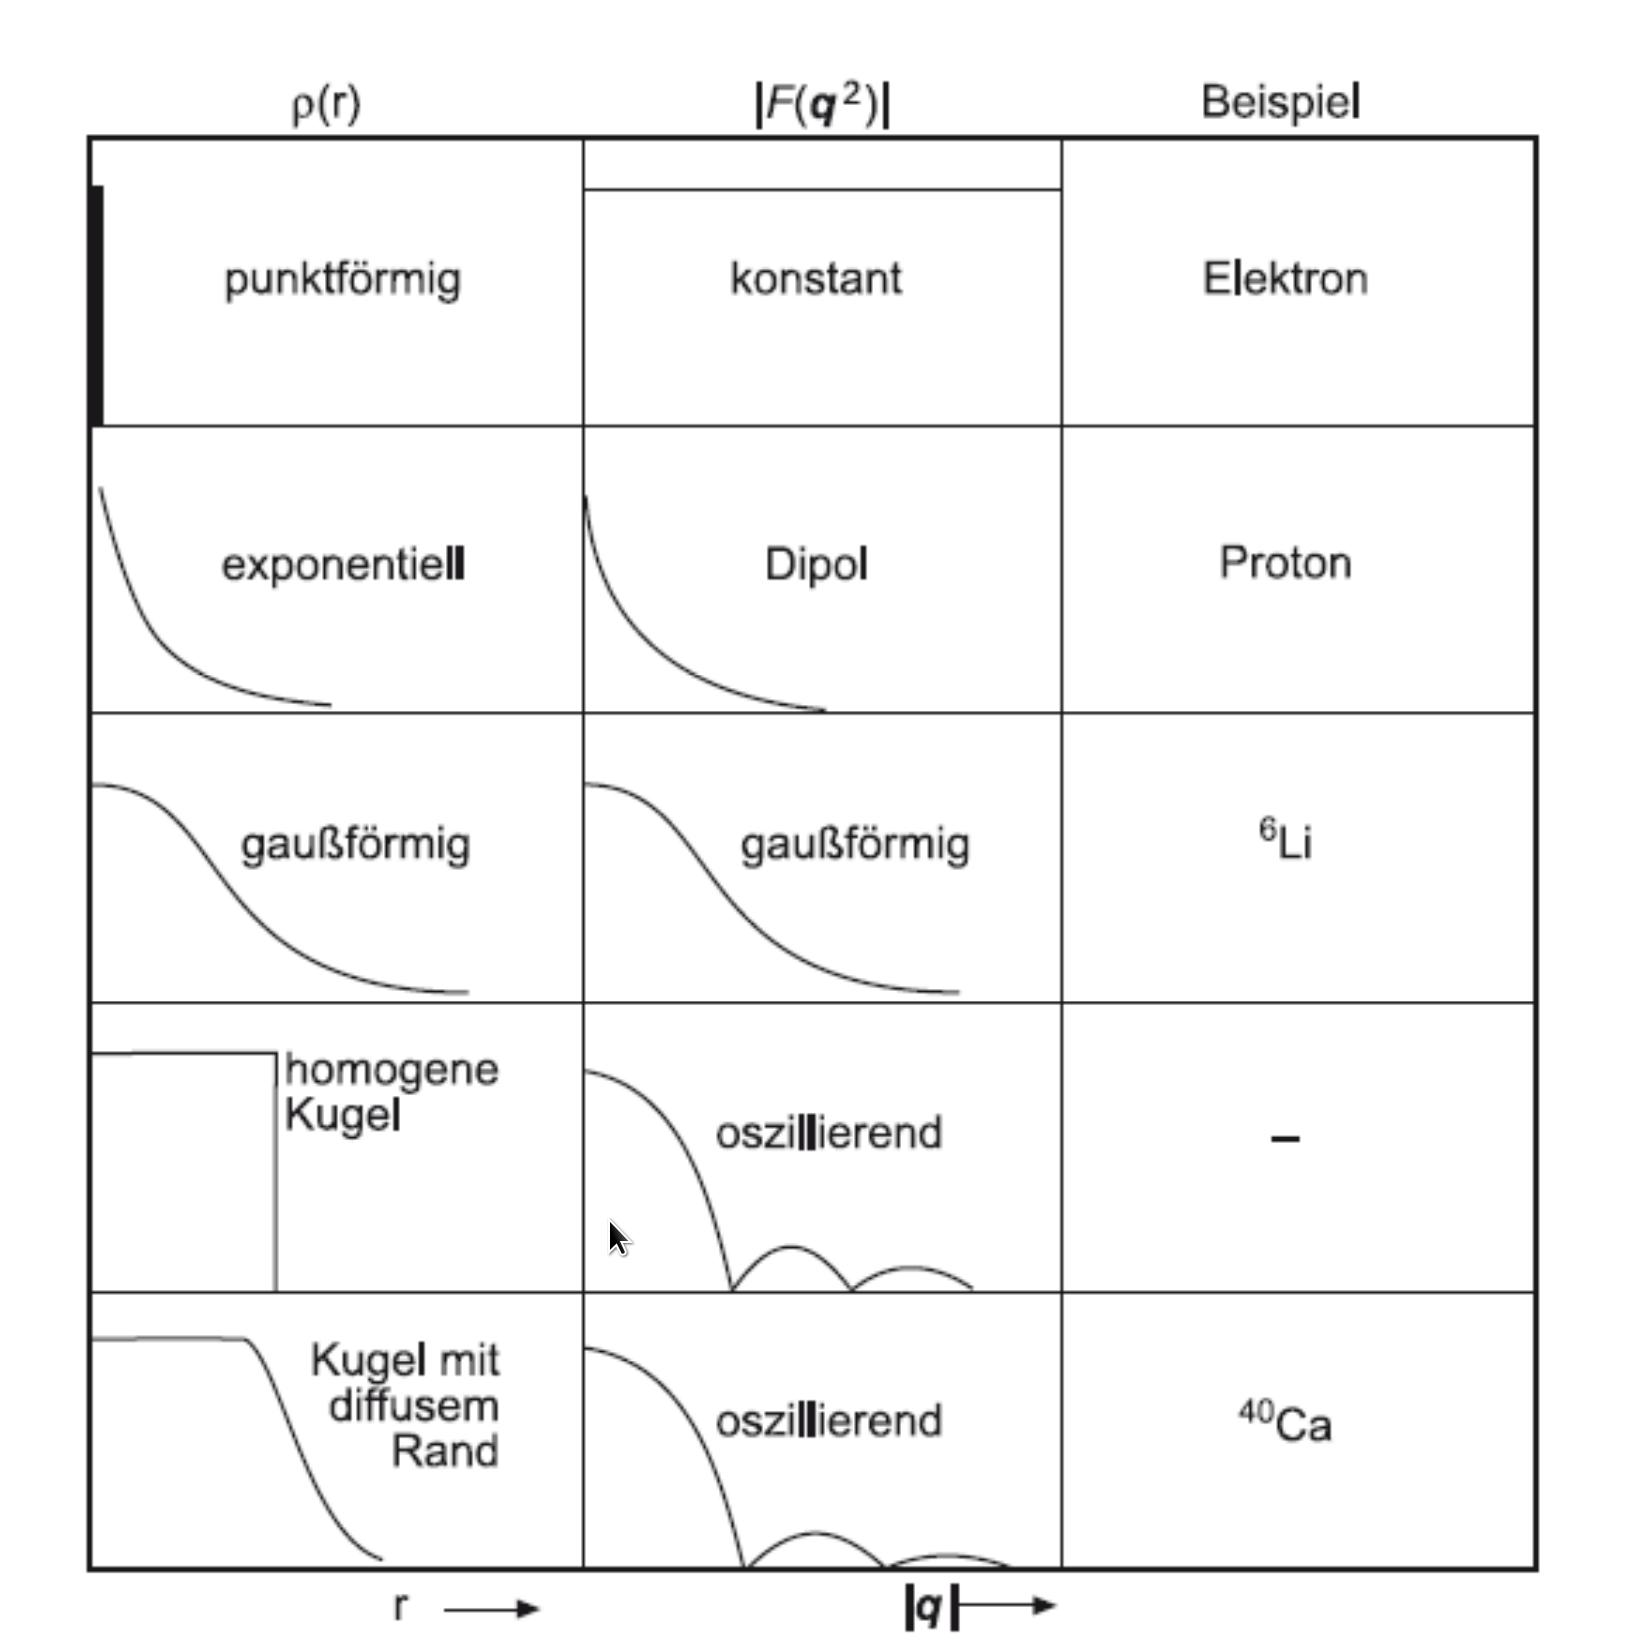
\includegraphics[width=.5\textwidth]{./img/formfaktoren_rho.jpeg}
	\caption{\textbf{Formfaktoren und zugehörige Ladungsverteilungen}}
	\label{fig:formfaktoren}
\end{figure}

\subsection{Formfaktoren}
In der Realität stellt man bei Streuexperimenten einen Unterschied zwischen dem theoretischen und gemessenen Mott-Wirkungsquerschnitt fest.
Dabei konvergieren die gemessenen Wirkungsquerschnitte nur für den Grenzfall verschwindender Impulsüberträge gegen den theoretischen Mott-Querschnitt und werden mit steigendem $|\mvec{q}|$ systematisch kleiner.
Der Grund hierfür ist, dass die Nukleonen und Kerne in Wirklichkeit ausgedehnte Objekte sind.
Somit ''sieht'' das Elektron bei der Streuung mit größerem $|\mvec{q}|$ nicht mehr die gesamte Ladung des Targets.
Der räumlichen Ausdehnung kann durch einen \textbf{Formfaktor $F(q^2)$} Rechnung getragen werden.
Da es bei kugelsymmetrischen Systemen keine Vorzugsrichtung gibt, hängt der Formfaktor dabei nur vom Betrag von $\mvec{q}$ ab.
Der Zusammenhang zwischen dem so angepassten Wirkungsquerschnitt und dem Mott-Wirkungsquerschnitt ist durch
\begin{equation*}
	\left(\diff[\sigma]{\Omega}\right)_\text{exp} = \left(\diff[\sigma]{\Omega}\right)_\text{exp}\cdot \left|F(q^2)\right|^2
\end{equation*}
gegeben.

Dabei kann in \textsc{Born}scher Näherung und unter Vernachlässigung des Targetrückstoßes der Formfaktor durch die Fouriertransformierte der Ladungsverteilung als
\begin{equation*}
	F(q^2) = \int{\text{d}^3x\ \rho(\mvec{x})e^{\frac{i}{\hbar}\mvec{q}\cdot\mvec{x}}}
\end{equation*}
ausgedrückt werden.

Theoretisch ließe sich durch inverse Fouriertransformation so Rückschluss auf die radiale Ladungsverteilung des Targets ziehen.
Dies ist in der Praxis jedoch nur beschränkt möglich, da der Wirkungsquerschnitt für steigende $|\mvec{q}|$ sehr schnell abnimmt und der Formfaktor generell nur über einen beschränkten Bereich bestimmt werden kann.
Dies resultiert daraus, dass der mögliche Impulsübertrag durch die Strahlenergie beschränkt ist.
Daher wählt man für gewöhnlich eine Parametrisierung von $\rho(r)$, bestimmt daraus den Formfaktor und variiert danach so lange die Parameter, bis die Modellfunktion mit den Messdaten übereinstimmt.
\autoref{fig:formfaktoren} zeigt Beispiele für verschiedene $\rho-F$ Paare.

\begin{figure}
	\centering
	\includegraphics[width=.5\textwidth]{./img/rosenbluth.pdf}
	\caption[Elektrischer und magnetischer Formfaktor von Proton und Neutron]{\textbf{Elektrischer und magnetischer Formfaktor von Proton und Neutron} aufgetragen gegen $Q^2$. Die Datenpunkte für $G_\text{M}^\text{n}$ und $G_\text{M}^\text{p}$ sind mit den angegebenen Faktoren skaliert und liegen dann übereinander}
	\label{fig:rosenbluth}
\end{figure}
Die Streuung eines Elektrons an einem Nukleon wird beispielsweise durch die \textbf{Rosenbluth-Formel}
\begin{equation*}
	\left(\diff[\sigma]{\Omega}\right)_\text{Rb} = \left(\diff[\sigma]{\Omega}\right)_\text{Mott}\cdot\left(\frac{G_\text{E}^2(Q^2) + \tau G_\text{M}^2(Q^2)}{1+\tau} + 2\tau\cdot G_\text{M}^2(Q^2)\tan^2\frac{\theta}{2}\right)
\end{equation*}
beschrieben. Es sind zwei Formfaktoren $G_\text{E}(Q^2)$ und $G_\text{M}(Q^2)$ nötig, um die elektrischen und magnetischen Verteilungen zu charakterisieren.
Sie hängen von $Q^2$ ab, daher kann man durch eine Messung der $Q^2$-Abhängigkeit auf die räumliche Verteilung von Ladung und magnetischem Moment schließen.
Im Grenzfall $Q^2\rightarrow 0$ entspricht dabei $G_\text{E}$ der auf die Elementarladung normierten elektrischen Ladung und $G_\text{M}$ dem auf das Kernmagneton normierten magnetischen Moment des Targets.
Man kann die Formfaktoren bestimmen, indem man den Wirkungsquerschnitt für jeweils feste Werte von $Q^2$ bei verschiedenen Streuwinkeln $\theta$ misst und durch den Mott-Querschnitt teilt.
Dann trägt man das Resultat gegen $\tan^2\frac{\theta}{2}$ auf, damit liegen die Messwerte auf einer Geraden, aus deren Achsabschnitt und Steigung sich die Formfaktoren bestimmen lassen.
\autoref{fig:rosenbluth} zeigt die Messung der Formfaktoren $G$ in Abhängigkeit des Impulsübertrages $Q^2$.

\section{Inelastische Kernanregungen}
\begin{figure}
	\centering
	\includegraphics[width=0.5\textwidth]{./img/inelastic.pdf}
	\caption{\textbf{Spektrum der Streuung an einem C-12 Kern}}
	\label{fig:inelastic}
\end{figure}
Nimmt man bei festem Streuwinkel $\theta$ ein Spektrum der gestreuten Elektronen auf, so registriert man Ereignisse nicht nur bei Energieüberträgen, die dem Rückstoß entsprechen,
sondern auch bei größeren.
Diese Ereignisse sind auf inelastische Reaktionen zurückzuführen.
\autoref{fig:inelastic} zeigt ein solches Spektrum.
Der Peak bei $E'\approx\SI{482}{\MeV}$ ist die elastische Streuung am C-Kern.
Unterhalb dieser Energie sieht man deutlich die Anregung einzelner Energieniveaus im Kern.

Über die Halbwertsbreite $\Gamma$ dieser Peaks lässt sich über die Unschärferelation
\begin{equation*}
	\underbrace{\Delta t}_{\equiv\tau}\cdot\underbrace{\Delta E}_{\equiv\Gamma} \geq \hbar\quad \Rightarrow\quad \Gamma = \frac{\hbar}{\tau}
\end{equation*}
die Lebensdauer $\tau$ solcher instabilen Zustände bestimmen.
Kann ein Zustand über verschiedene Kanäle zerfallen, so ist die totale Zerfallsbreite näherungsweise die Summe der partiellen Zerfallsbreiten
\begin{equation*}
	\Gamma_\text{tot} = \sum_i \Gamma_i.
\end{equation*}

Die Wellenfunktion eines zerfallenden Zustandes kann geschrieben werden als
\begin{equation*}
	\psi(t) = \psi_0e^{-\frac{i}{\hbar}\left(E_\text{R}-i\frac{\Gamma}{2}\right)t}.
\end{equation*}
Das fouriertransformierte Amplitudenquadrat $P(E)$ ergibt damit die Energieverteilung eines instabilen Zustandes
\begin{equation*}
	P(E) = \psi^*\psi\propto \frac{\hbar^2\Gamma^2}{(E_\text{R}-E)^2+\frac{\Gamma^2}{4}}.
\end{equation*}
Man nennt diesen Zusammenhang die \textbf{Breit-Wigner-Resonanzformel}.

	\chapter{Tiefinelastische Streuung}
Um die Substruktur zusammengesetzter Teilchen zu erforschen, braucht man eine gute Auflösung.
Dabei muss die Wellenlänge der ausgetauschten, virtuellen Photonen viel kleiner als die räumliche Ausdehnung des Nukelons sein
\begin{equation*}
	\frac{\lambda}{2\pi}\ll R\quad\Rightarrow\quad Q^2 \gg \left(\frac{\hbar}{R}\right)^2.
\end{equation*}
Derartig große Impulsüberträge fordern hohe Strahlenergien.
Die ersten Experimente dieser Art wurden in den 70ern am SLAC durchgeführt, einem Linearbeschleuniger für Elektronen mit ca. \SI{25}{\GeV}.
Bei der zweiten Generation dieser Experimente, welche in den 80ern am CERN und FNAL stattfanden, wurden Myonen anstelle von Elektronen verwendet.
Diese verhalten sich in jeder Hinsicht wie Elektronen, da sie geladene, punktförmige Teilchen mit Spin-$\nicefrac{1}{2}$ sind.
Allerdings bieten Myonen den Vorteil, mit größeren Energien erzeugt werden zu können.
Man beschießt dazu Targets mit hochenergetischen Protonen, wobei viele Pionen entstehen.
Ein Teil dieser Pionen zerfällt auf dem Flug in Myonen.
Diese Werden nach Impulsen selektiert und mit Magnetlinsen zu einem Strahl gebündelt.
So ließen sich am CERN Strahlenergien von bis zu \SI{280}{\GeV} erzeugen, am FNAL sogar \SI{490}{\GeV}.
Die letzte Generation wurde am HERA-Speicherring realisiert.
Dort zirkulieren Elektronen bzw. Positronen mit einer Energie von \SI{27.6}{\GeV} und Protonen mit einer maximalen Energie von \SI{920}{\GeV} in separaten Speicherringen und werden an einer Stelle zur Kollision gebracht.
Damit lassen sich Strahlenergien im fünfstelligen \si{\GeV}-Bereich erreichen.

	\chapter{Quarks, Gluonen und die starke Wechselwirkung}

\section{Quarks in Hadronen}
Neben den Nukleonen gibt es noch viele instabile Hadronen.
Man teilt Hadronen in zwei Klassen auf:
\begin{itemize}
	\item \textbf{Baryonen} \begin{itemize}
		\item halbzahliger Spin, daher Fermionen
		\item Protonen, Neutronen\dots
	\end{itemize}
	\item \textbf{Mesonen} \begin{itemize}
		\item ganzzahliger Spin, daher Bosonen
		\item Pionen, Kaonen,\dots
	\end{itemize}
\end{itemize}

\subsection{Baryonen}
Alle Baryonen sind aus \textbf{3 Quarks} zusammengesetzt.
Da die Quarks Spin $\tfrac{1}{2}$ haben, ergibt sich daraus der halbzahlige Baryonen-Spin.
Wenn in Teilchenreaktionen zusätzliche Baryonen erzeugt werden, dann wird zugleich die gleiche Zahl an Antibaryonen erzeugt.
Zur Beschreibung führt man die additive \textbf{Baryonenzahl $B$} ein.
Sie beträgt 1 für alle Baryonen und -1 für alle Antibaryonen.
(Anti)Quarks haben demnach die Baryonenzahl ($-$)$\tfrac{1}{3}$.

\textbf{Die Baryonenzahl ist in jeden bekannten Teilchenreaktionen eine Erhaltungsgröße.}

\subsection{Mesonen}
Hadronen aus Quark-Antiquark-Paaren nennt man \textbf{Mesonen}.
Ihr ganzzahliger Spin setzt sich aus der Spinkopplung des Quarkpaares und etwaigen ganzzahligen Bahndrehimpulsen zusammen.
Es gibt keine Mesonenzahlerhaltung.
Dies ergibt Sinn, da Mesonen Quark-Antiquark-Kombinationen sind (ihre Baryonenzahl somit 0 ist), wodurch beliebig viele Mesonen erzeugt werden können ohne die Baryonenzahlerhaltung zu verletzen.

\section{Quark-Gluon-Wechselwirkung}
\subsection{Die Farbe}
Die \textbf{Farbe} wird benötigt, um das Pauli-Prinzip für die Quarks der Hadronen zu gewährleisten.

Betrachten wir beispielsweise die $\Delta^{++}$-Resonanz.
Der Spin dieses Baryons beträgt $J=\nicefrac{3}{2}$ und die Parität ist positiv.
Da das $\Delta^{++}$ das leichteste Baryon mit $J^P=\nicefrac{3}{2}^+$ ist, kann man annehmen, dass der Bahndrehimpuls verschwindet, die Ortswellenfunktion somit symmetrisch ist.
Damit sich der Spin von $\tfrac{3}{2}$ ergibt, müssen alle Spins parallel sein.
Damit ist auch die Spinwellenfunktion symmetrisch.
Ferner ist die Wellenfunktion auch unter Vertauschung zweier Quarks symmetrisch, da nur Quarks derselben Sorte vorhanden sind.
Damit scheint die Gesamtwellenfunktion symmetrisch zu sein, was aber gegen das Pauli-Prinzip verstößt.

Es lässt sich allerdings dadurch retten, indem man eine neue Quantenzahl einführt: Die \textbf{Farbe}.
Sie kann drei Werte (rot, blau, grün) annehmen.
Entsprechend gibt es für Antiquarks auch Farben (antirot, antiblau, antigrün).
Hiermit kann man eine unter Quarkvertauschung antisymmetrische Farbwellenfunktion konstruieren, sodass die Gesamtwellenfunktion antisymmetrisch ist

	\chapter{Elektron-Positron-Kollisionen}
\section{Allgemeines}
In der Elektron-Positron-Annihilation können alle schwach und elektromagnetisch Wechselwirkenden Teilchen erzeugt werden.
Austauschbosonen sind in diesem Fall entweder das Photon $\gamma$ oder das $Z^0$-Boson.
Da Neutrinos elektrisch ungeladen sind, können Neutrino-Antineutrino-Paare nur durch den Austausch eines $Z^0$ erzeugt werden.

In einem Speicherring mit kollidierenden Teilchen gleicher Energie beträgt die maximale Schwerpunktsenergie $\sqrt{s}=2E$, womit alle Teilchen-Antiteilchen-Paare der Massen $2m = \nicefrac{\sqrt{s}}{c^2}$ erzeugt werden können.
Anders als bei Fixed-Target-Experimenten steht in Collider-Experimenten die gesamte Schwerpunktsenergie zur Verfügung, während im anderen Fall nur $s\approx 2MEc^2$ genutzt werden können, die Schwerpunktsenergie wächst also nur mit der Wurzel der Strahlenergie.

\section{Erzeugung von Leptonenpaaren}
\subsection{Myonen}
Sie sind die leichtesten Teilchen, die in $\el\pos$-Reaktionen erzeugt werden können:
\begin{equation*}
	\el + \pos \rightarrow \mu^- + \mu^+.
\end{equation*}
Myonen haben eine Masse von \SI{105.7}{\MeV} und durchdringen Materie aufgrund ihrer vergleichsweise hohen Masse und der fehlenden starken Wechselwirkung sehr leicht.
Mit $\tau=\SI{2}{\micro\second}$ haben Myonen nach den Neutronen die längste Lebensdauer aller instabiler Elementarteilchen.
\newpage
\subsection{Tauonen}
Wir die Schwerpunktsenergie weiter erhöht, so können $\tau^-\tau^+$-Paare erzeugt werden.
Diese sind aber mit $\tau=\SI{3e-13}{\second}$ deutlich kurzlebiger als ihre Myon-Kollegen, weshalb sie in Detektoren nur über ihre Zerfallsprodukte nachgewiesen werden können:
\begin{figure}[h!]
	\centering
	\includegraphics[width=.8\textwidth]{./img/tauon-prod.pdf}
\end{figure}
Die dabei entstehenden Neutrinos sind in der Regel nicht nachweisbar.
Die Masse der Tauonen beträgt \SI{1777}{\GeV}.

\subsection{Bhabha-Streuung}
\begin{figure}
	\centering
	\includegraphics[width=.7\textwidth]{./img/bhabhaprocesses.pdf}
	\caption{Links: $\el\pos$-Streuung, Rechts: Paarvernichtung/-erzeugung}
	\label{fig:bhabha}
\end{figure}
\begin{figure}
	\centering
	\includegraphics[width=.7\textwidth]{./img/bhabhacross.pdf}
	\caption{Wirkungsquerschnitt der $\el\pos$-Reaktionen}
	\label{fig:crossbhabha}
\end{figure}
Die Erzeugung geladener Leptonenpaare kann näherungsweise als rein elektromagnetischer Prozess angesehen werden.
Die elastische Streuung $\el\pos\rightarrow\el\pos$ nennt sich auch \textbf{Bhabha-Streuung}.
Sowohl die $\el\pos$-Paarvernichtung mit anschließender Erzeugung eines $\el\pos$-Paares aus einem virtuellen Photon, als auch die bloße Streuung von Elektron und Positron aneinander führen dabei zum gleichen Endzustand, wie in \autoref{fig:bhabha} zu sehen ist.
Daher müssen bei der Berechnung des Wirkungsquerschnittes beide Feynman-Amplituden addiert werden.
Die Myon-Antimyon-Erzeugung ist einfacher zu berechnen und der differenzielle Wirkungsquerschnitt lautet
\begin{equation*}
	\diff[\sigma]{\Omega} = \frac{(\alpha\hbar c)^2}{4s}\cdot(1+\cos^2\theta).
\end{equation*}
Die übrigen $\el\pos$-Reaktionen werden auf diesen (totalen) Wirkungsquerschnitt normiert.

In \autoref{fig:crossbhabha} sind die Wirkungsquerschnitte beider besprochenen Reaktionen abgebildet.
Ist die Schwerpunktsenergie ausreichend hoch, sodass die Ruhemassen der beteiligten Teilchen vernachlässigt werden können, so ergibt sich ein nahezu identischer Wirkungsquerschnitt für Tauonen und Myonen.
Dieses Phänomen wird als \textbf{Leptonenuniversalität} bezeichnet und meint, dass sich Elektronen, Myonen und Tauonen abgesehen von ihrer Masse gleich verhalten.

Da die obige Formel für den Wirkungsquerschnitt die Messdaten gut reproduziert, ist der Formfaktor dieser Reaktion Eins.
Dies bedeutet, dass diese Leptonen in der Tat punktförmige Teilchen sind.

\subsection{Resonanzen}
Betrachtet man den Wirkungsquerschnitt für die Erzeugung von Myonenpaaren und Hadronen in $\el\pos$-Streuung, so findet man jeweils die $\nicefrac{1}{s}$.
Dieser Funktion sind im hadronischen Ausgangskanal ausgeprägte Maxima überlagert, die man \textbf{Resonanzen} nennt.
Man kann diesen Resonanzen wie bei ordinären Teilchen eine Masse und Quantenzahlen zuweisen.
\autoref{fig:resonances} zeigt verschiedene Resonanz-Peaks.

\subsection{Nichtresonante Erzeugung von Hadronen}
Selbstverständlich können auch zwischen den Peaks Quark-Antiquark-Paare erzeugt werden.
An die Primärquark-Antiquarks lagern sich dabei weitere Quark-Antiquark-Paare an und es entstehen Hadronen.
Diesen Vorgang nennt man \textbf{Hadronisierung}.
Natürlich können dabei nur Teilchen hadronisiert werden, deren Masse kleiner als die halbe zur Verfügung stehende Schwerpunktsenergie ist.
Im Gegensatz zu Leptonen tragen die Quarks nicht eine volle Elementarladung, sondern nur drittelzahlige Ladungen $z_\text{q}\cdot\text{e}$, die vom jeweiligen Quark-Flavor abhängig sind.
Da es ebenfalls 3 verschiedene Farbzustände gibt, geht in den Wirkungsquerschnitt noch der Faktor 3 mit ein.
Normiert man nun den Wirkungsquerschnitt des hadronischen Kanals mit dem Myonpaar-Wirkungsquerschnitt, so ergibt sich das Verhältnis
\begin{equation*}
	R=\frac{\sum_q\sigma(\el\pos\rightarrowq\bar{q})}{\sigma(\el\pos\rightarrow\mu^-\mu^+)} = 3\cdot\sum_qz_\text{q}^2,
\end{equation*}
welcher experimentell sehr leicht durch $\el\pos$-Kollisionen zugänglich ist.
Summiert werden bei obiger Formel nur die Ladungen der Quarks, für deren Erzeugung die Schwerpunktsenergie ausreicht.
Diese Messung ist eine eindrucksvolle Bestätigung dafür, dass es genau 3 Farben gibt, denn bei obiger Herleitung wurde vorausgesetzt, dass es 3 Farben gibt, was die Messdaten hervorragend reproduziert.

	\chapter{Phänomenologie der schwachen Wechselwirkung}
Die schwache Wechselwirkung ist für den Zerfall von Quarks und Leptonen verantwortlich.
Es sind keine gebundenen Zustände bekannt, die sich aufgrund der schwachen Wechselwirkung bilden.
In Streuexperimenten ist die schwache Wechselwirkung nur schwer beobachtbar, da alle Teilchenreaktionen, die der schwachen Wechselwirkung unterliegen, sehr geringe Wirkungsquerschnitte haben.

\section{Leptonen}
Wie bereits in den vorigen Kapiteln gesehen, gibt es \textbf{3 Leptonenfamilien}:
\begin{equation*}
	\twovec{\nu_e}{\el}\quad\twovec{\nu_\mu}{\mu^-}\quad\twovec{\nu_\tau}{\tau^-}.
\end{equation*}
Wie die Quarks unterscheiden sich auch die geladenen Leptonen deutlich in ihrer Masse.

\section{Typen der schwachen Wechselwirkung}
Es gibt zwei Typen der schwachen Wechselwirkung, nämlich die Wechselwirkung mit einem
\begin{itemize}
	\item \textbf{neutralen Strom} unter Austausch eines $Z^0$-Bosons, der die Flavors der Quarks und die Leptonen unverändert lässt und Wechselwirkungen mit einem
	\item \textbf{geladenen Strom} unter Austausch eines $W^+$- oder $W^-$-Bosons, der flavorändernd wirken kann.
\end{itemize}

Die erwähnten Austauschbosonen sind Vektorbosonen (Spin-1-Teilchen).

\section{Geladene Ströme}
Man kann geladene Ströme in 3 Klassen unterteilen: in \textit{leptonische}, \textit{semileptonische} und \textit{nichtleptonische Prozesse}.

	\chcapter{Elektroschwache Theorie}

\section{Reele W- und Z-Bosonen}
In $\el\pos$-Collidern ist zur Erzeugung von $Z^0$-Bosonen gemäß
\begin{equation*}
	\el + \pos \rightarrow Z^0
\end{equation*}
eine Schwerpunktsenergie von $\sqrt{s}=M_\text{Z}c^2$ erforderlich.
W-Bosonen können aufgrund der Ladungserhaltung nur in Paaren erzeugt werden
\begin{equation*}
	\el + \pos \rightarrow W^+ + W^-,
\end{equation*}
weshalb auch höhere Schwerpunktsenergien nötig sind.

Für viele Jahre bestand die einzige Möglichkeit für die Erzeugung der Bosonen darin,
die Quarks im Proton auszunutzen, gemäß
\begin{alignat*}{2}
	u + \bar{u} &\rightarrow Z^0 \quad d + \bar{u} &\rightarrow W^- \\
	d + \bar{d} &\rightarrow Z^0 \quad u + \bar{d} &\rightarrow W^+.
\end{alignat*}
Anstatt aber bloß zwei Protonen frontal kollidieren zu lassen und auf die Anti-Seequarks zu hoffen (relativer Anteil im Proton im Mittel $\approx 0.04$),
lässt man lieber Protonen und Antiprotonen kollidieren, wodurch man deutlich weniger Schwerpunktsenergie im Mittel benötigt.

Die Bosonen können dann durch die Zerfälle
\begin{alignat*}{2}
	Z^0 &\rightarrow \el\pos \quad W^+ \rightarrow \pos + \nu_\text{e} \\
	Z^0 &\rightarrow \mu^-\mu^ \quad W^+ \rightarrow \mu^+ + \nu_\text{\mu}.
\end{alignat*}
Experimentell beobachtet man also ein hochenergetisches $\el\pos$- oder $\mu^-\mu^+$-Paar, wobei Lepton und Antilepton in entgegengesetzten Richtungen wegfliegen müssen.

	\chapter{Eichtransformationen}
\section{Lagrangedichte}
Im Rahmen einer klassischen Feldtheorie kann die Dynamik eines Systemes mit der Lagrangedichte $\mathcal{L}$ beschrieben werden.
Aus ihr können durch die Euler-Lagrange-Gleichung Bewegungsgleichungen des Systemes hergeleitet werden.
Für ein Klein-Gordon-Feld gilt
\begin{equation*}
	\mathcal{L} = \partial_\mu\phi\partial^\mu\phi^* - m^2\phi\phi^*
\end{equation*}
und für ein Dirac-Feld
\begin{equation*}
	\mathcal{L} = \bar{\psi}(i\gamma^\mu\partial_\mu - m)\psi.
\end{equation*}
Wendet man auf diese Lagrangedichten Euler-Lagrange-Gleichungen
\begin{equation*}
	\partial^\mu\frac{\partial\mathcal{L}}{\partial(\partial^\mu\phi_i)}-\frac{\partial\mathcal{L}}{\partial\phi_i}
\end{equation*}
an, so erhält man bei Bosonen die Klein-Gordon-Gleichung und bei Fermionen die Dirac-Gleichung.

\section{Globale und lokale Phasentransformationen}
Die Lagrangedichten sollten so konstruiert sein, dass sie kovariant unter globalen und lokalen Phasentransformationen sind.
Eine solche Transformation lautet für globale Phasen
\begin{alignat*}{3}
	\psi(x,t) &\rightarrow \psi'(x,t) &&= e^{i\theta}\psi(x,t) \\
	\bar{\psi}(x,t) &\rightarrow\bar{\psi}'(x,t) &&= \bar{\psi}(x,t)e^{-i\theta}.
\end{alignat*}
Für lokale Phasen $\theta=\theta(x,t)$ muss in der Lagrangedichte die Ableitung $\partial_\mu$ durch eine kovariante Ableitung
\begin{equation*}
D_\mu\rightarrow D'_\mu = D_\mu - i\partial_\mu\theta	\quad\text{mit}\ D_\mu=\partial_\mu + ieA_\mu
\end{equation*}
ersetzt werden, damit die betroffene Lagrangedichte kovariant bleibt.
Das Transformationsverhalten des Eichfeldes muss dann $A_\mu\rightarrow A'_\mu=A_\mu-\frac{1}{e}\partial_\mu\theta$ lauten, was bereits aus der Elektrodynamik bekannt ist.

Man kann also für das Feld $\psi(x,t)$ eine beliebige Phase $\theta(x,t)$ erlauben, solange man ein vermittelndes Feld $A_\mu$ einführt, das diese Information von $(x,t)$ zu $(x',t')$ transportiert.
Das Eichfeld $A_\mu$ koppelt dabei an die Größe $e$ des Feldes $\psi(x,t)$.

Die Einführung dieses Eichfeldes führt bei einem Fermion zum Beispiel zu einem weiteren Wechselwirkungssektor
\begin{equation*}
	\mathcal{L}_\text{IA} = \underbrace{\bar{\psi}(i\gamma^\mu\partial_\mu - m)\psi}_\text{frei} - \underbrace{e\bar{\psi}\gamma^\mu\ \textcolor{red}{A_\mu}\ \psi}_\text{IA}.
\end{equation*}

	\chapter{Diskrete Symmetrien und Erhaltungssätze}
\section{Diskrete Symmetrien}
\begin{figure}[h!]
	\centering
	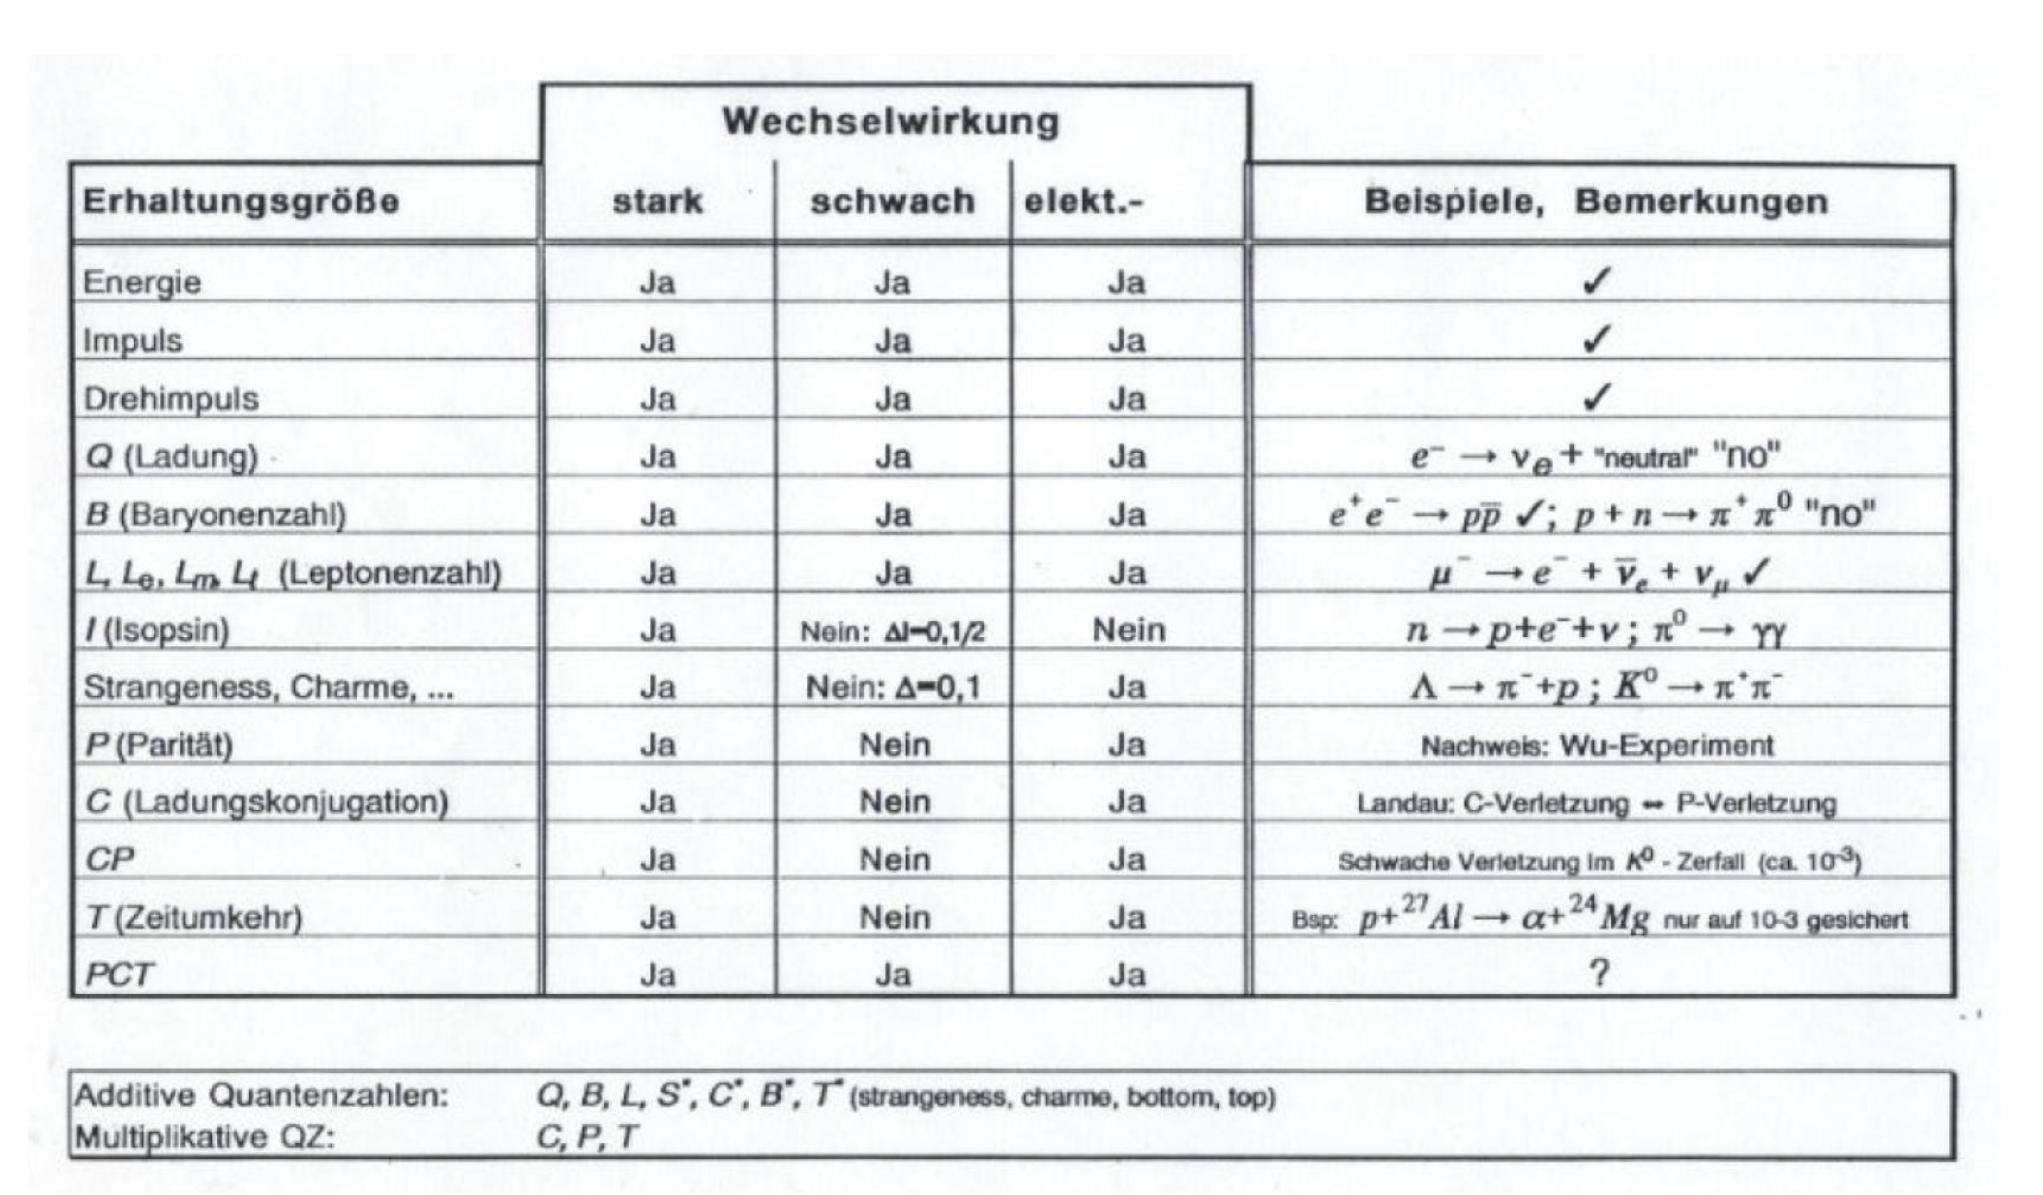
\includegraphics[width=.7\textwidth]{./img/symmetries.jpg}
	\caption{Zusammenfassung der Erhaltungsgrößen}
	\label{fig:symmetries}
\end{figure}

\section{Parität}
\subsection{Der $\mathcal{P}$-Operator}
Der Paritätsoperator $P$ erzeugt eine räumliche Spiegelung im Ursprung.
Sie ist eine mulitplikative Quantenzahl mit den möglichen Eigenwerten $\pm 1$.
Eine Reaktion $a+b\longrightarrow c+d$ hätte die Gesamtparität
\begin{equation*}
	P_a\cdot P_b\cdot (-1)^l = P_c\cdot P_d\cdot (-1)^{l'}
\end{equation*}
mit etwaigen Bahndrehimpulsen $l,l'$.
Dabei sind $P_i$ die \textbf{Eigenparitäten} der Teilchen.
Man definiert:
\begin{align*}
	P(q) &= -P(\bar{q}) = 1 \\
	P(p) &= P(n) = P(\Lambda) = 1
\end{align*}
Außerdem haben bei \textbf{Fermionen} Teilchen und Antiteilchen \textbf{entgegengesetzte} Parität,
bei \textbf{Bosonen} jedoch \textbf{gleiche} Parität.

Alle anderen Paritäten lassen sich daraus ableiten.

\subsection{Paritätsverletzung durch die schwache Wechselwirkung}
Eine einzigartige Eigenschaft der schwachen Wechselwirkung ist die, paritätsverletzend zu sein.
Reaktionen der schwachen Wechselwirkung sind nicht spiegelsymmetrisch.
Dies folgt aus der experimentell belegten Tatsache, dass die schwache Wechselwirkung eine Wechselwirkung mit Axial- und Vektorcharakter zugleich ist.
Die Stärke der Axialvektor- und Vektoranteile werden dabei durch zwei Koeffizienten $c_\text{A}$ und $c_\text{V}$ beschrieben.
Bei einer V+A-Wechselwirkung ($c_\text{V}=c_\text{A}$) koppelt die Wechselwirkung nur an rechtshändige Fermionen und linkshändige Antifermionen.
Bei einer V-A-Wechselwirkung ($c_\text{V}=-c_\text{A}$) koppelt die Wechselwirkung nur an linkshändige Fermionen und rechtshändige Antifermionen.
Für die Kopplungsstärke der W-Bosonen findet man $c_\text{V}=-c_\text{A}=1$.
Man spricht daher auch von einer V-A-Theorie der geladenen Ströme.
Die Parität ist \textbf{maximal verletzt}, wenn gilt: $|c_\text{V}|=|c_\text{A}|$, was bei geladenen Strömen zutrifft.

\begin{figure}
	\centering
	\includegraphics[width=.5\textwidth]{./img/myondecay.pdf}
	\caption{Myonzerfall, eine Möglichkeit ist unterdrückt}
	\label{fig:myondecay}
\end{figure}
Ein Beispiel für die Paritätsverletzung der schwachen Wechselwirkung ist der Myonzerfall $\mu^-\rightarrow\el + \nu_\mu + \bar{\nu}_e$ (\autoref{fig:myondecay}).
Im Ruhesystem des Myons hat das Elektron den größten Impuls, wenn die Impulse der Neutrinos parallel zueinander und entgegengesetzt zur Impulsrichtung des Elektrons stehen.
Da sich die Spins des $\nu\bar{\nu}$-Paares aufheben müssen, muss der Spin des Elektrons dem Spin des Myons gleichgerichtet sein, um Spinerhaltung zu erfüllen.
Experimentell beobachtet man, dass Elektronen aus dem Myonzerfall allerdings bevorzugt linkshändig emittiert werden!
Somit ist die Parität maximal verletzt.

\subsection{Das Wu-Experiment}
\begin{figure}
	\centering
	\begin{subfigure}{0.5\textwidth}
		\centering
		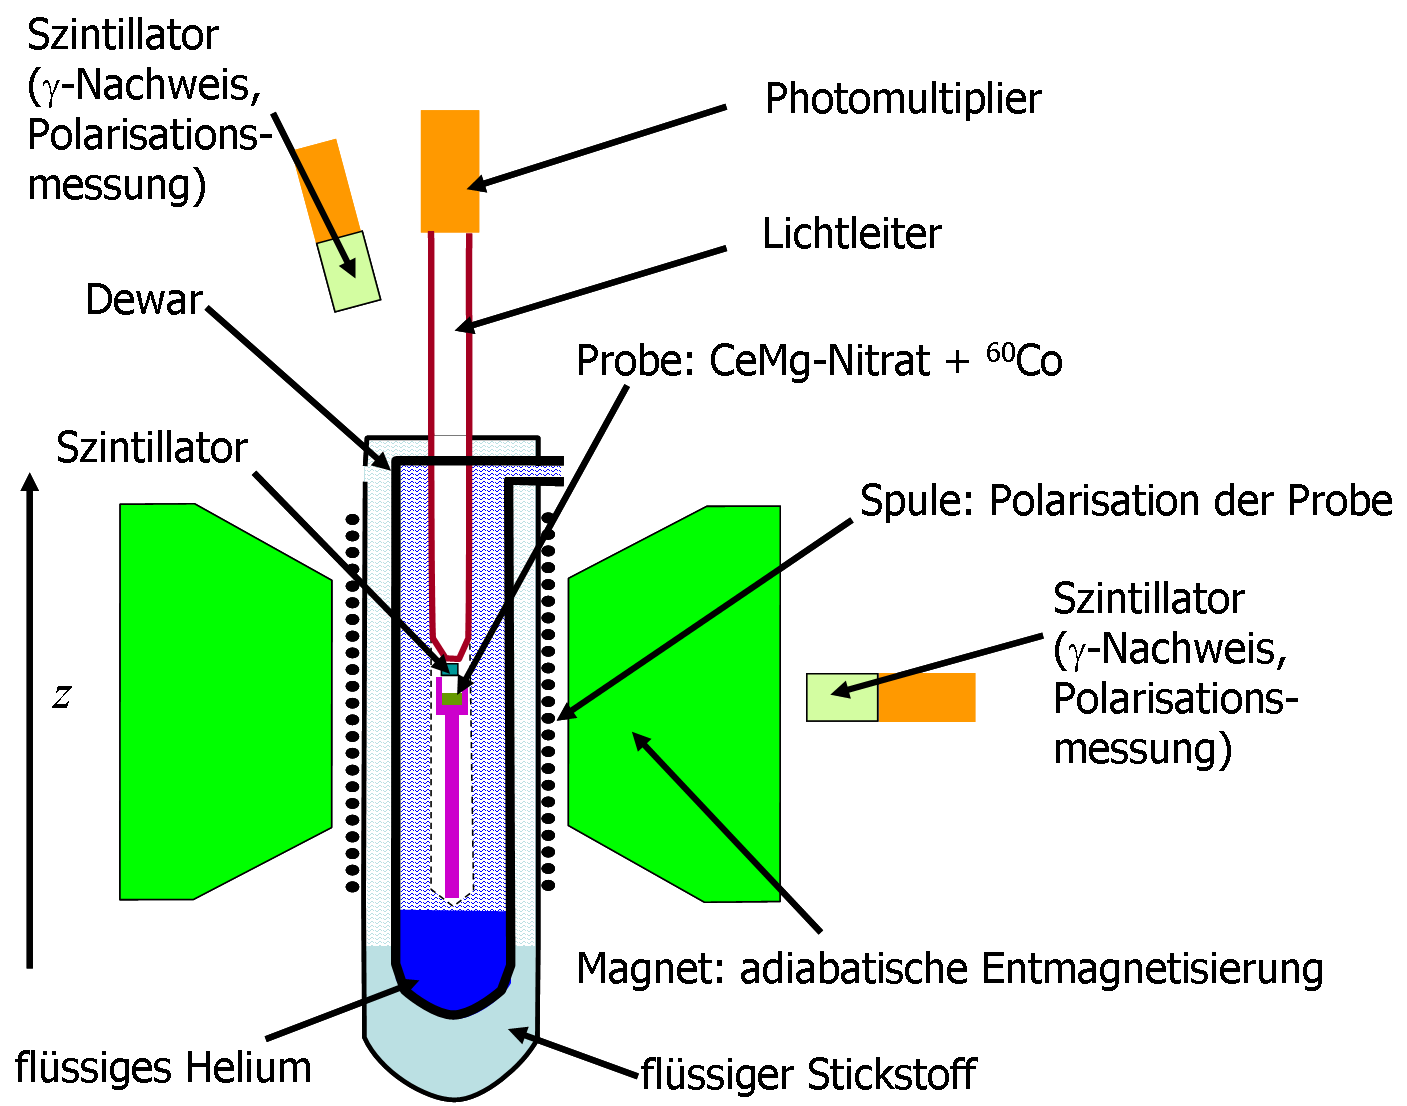
\includegraphics[width=.5\textwidth]{./img/wu.jpg}
		\caption{Das Wu-Experiment: Detektor in negativer z-Richtung}
		\label{fig:wu}
	\end{subfigure}
	\begin{subfigure}{0.4\textwidth}
		\centering
		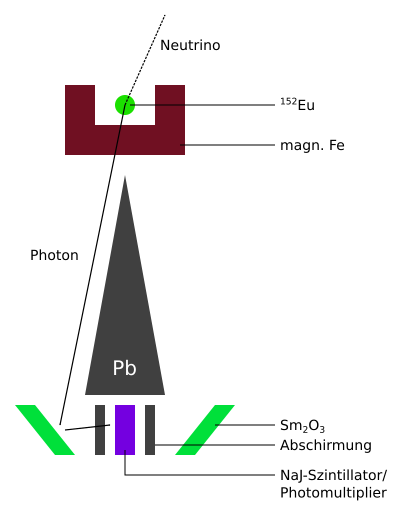
\includegraphics[width=.5\textwidth]{./img/gold.pdf}
		\caption{Das Goldhaber-Experiment: Target unten, Quelle oben}
		\label{fig:gold}
	\end{subfigure}
	\caption{Experimente zur Untersuchung der Paritätsverletzung}
\end{figure}
Eindrucksvoll konnte das Wu-Experiment die Paritätsverletzung der schwachen Wechselwirkung demonstrieren.
Es wurde der Kern-$\upbeta$-Zerfall von $^{60}Co$ untersucht.
Der Versuchsaufbau ist in \autoref{fig:wu} zu sehen.
Die Fragestellung war, ob es eine Vorzugsrichtung der beim $\upbeta$-Zerfall emittierten Elektronen relativ zum Spin des $^{60}Co$-Kerns gibt.
Die Reaktion lautet
\begin{equation*}
	Co(5+)\longrightarrow Ni^*(4+) + \el + \bar{\nu}_e.
\end{equation*}
Die technische Herausforderung dabei war, die Ausrichtung des Spins der Co-Kerne bei sehr tiefen Temperaturen.
Man verwendete das Prinzip der ’’adiabatischen Entmagnetisierung’’ ($\rightarrow$ \url{de.wikipedia.org/wiki/Magnetische_K%C3%BChlung}).

Es wird nun mit einem Detektor in negativer z-Richtung die Anzahl der emittierten Elektronen gemessen, einmal mit Magnetfeld in z-Richtung, einmal in -z-Richtung(, was einer Paritätsumkehr entspricht).
Man stellt fest, dass deutlich mehr Elektronen mit Spin antiparallel zur Spinrichtung der Kerne emittiert werden, als parallel dazu.
Dies ist die Bestätigung der maximalen Paritätsverletzung in der schwachen Wechselwirkung.

\subsection{Das Goldhaber-Experiment}
Das Goldhaber-Experiment zeigt nun sogar, dass es nur linkshändige Neutrinos und rechtshändige Antineutrinos gibt.
Betrachtet wird der Zerfall von Eu-152-Kernen in einem metastabilen Zustand durch K-Einfang
\begin{equation*}
	Eu\text{(meta)} + \el \longrightarrow Sm^* + \nu_e.
\end{equation*}
Der Tochterkern befindet sich in einem angeregten Zustand, der danach durch $\upgamma$-Emission relaxiert.
Dabei erfüllt die Zerfallskaskade folgende Eigenschaften:
\begin{itemize}
	\item Spinfolge $0^-\rightarrow 1^-\rightarrow 0^+$
	\item gleiche Übergangsenergien (ca. 1\% Abweichung der Energien)
	\item Sehr kurze Lebensdauer des Sm ($\approx\SI{3e-14}{\second}$).
\end{itemize}
\autoref{fig:gold} zeigt den Versuchsaufbau.
Der Nachweis der Gamma-Quanten aus dem Sm-Zerfall beruht auf der resonanten Streuung der Gamma-Quanten an einem Sm2O3-Target, welches ringförmig um den Detektor angebracht ist.
Die Bleiabschirmung hindert Zerfallsphotonen aus der Eu-152-Quelle daran, den Detektor direkt zu erreichen.
Die resonante Streuung findet über Kernresonanzabsorption des Photons durch einen Sm-Kern und anschließende spontane Emission statt.
Da die Quellkerne kurze Zeit zuvor ein Neutrino abgegeben haben, ist der angeregte Sm-Kern nicht in Ruhe.
Somit hat das Relaxationsphoton genügend Energie, um resonant absorbiert zu werden und der angeregte Sm-Zustand eine ausreichend geringe Lebensdauer, um nicht durch Wechselwirkungen mit dem Gitter zu relaxieren.
Dieser Trick funktioniert allerdings nur, wenn das Neutrino nach oben emittiert wurde, andernfalls ist die Energiedifferenz zu hoch.
Damit kann also die Richtung der Neutrinoemission bestimmt werden.

Durch einfache Spinbetrachtungen gelangt man zum Schluss, dass die Helizität der Relaxationsphotonen der der emittierten Neutrinos entsprechen muss.
Der Detektor wird von einem magnetisierten Eisenblock abgeschirmt, sodass etwa 7-8\% der Elektronen im Eisen polarisiert sind.
Die Compton-Streuung der Relaxationsphotonen mit den Elektronen im Eisenblock hängt stark von der Polarisierung des streuenden Materials ab.
Falls es eine Vorzugsrichtung der Helizität der Photonen und damit der Neutrinos geben sollte, so müssten sich die Zählraten je nach Magnetisierungsrichtung des Eisenblocks stark unterscheiden.
Tatsächlich misst man nur in eine Magnetisierungsrichtung Ereignisse.

Somit ist bestätigt, dass Neutrinos nur linkshändig vorkommen.

\section{Ladungskonjugation}
\subsection{Der $\mathcal{C}$-Operator}
Der C-Operator führt in einem System Teilchen in Antiteilchen und vice versa über.

\subsection{CP-Erhaltung}
Man kann leicht sehen, dass durch die festgelegte Helizität der Neutrinos die schwache Wechselwirkung C-Symmetrie von vornherein bricht (C auf linkshändiges Neutrino $\rightarrow$ linkshändiges Antineutrino, gibt's aber im SM nicht!).
Wendet man jedoch CP gemeinsam auf Prozesse an, an denen die schwache Wechselwirkung beteiligt ist, so entstehen Prozesse, die in der Natur existieren.
Die schwache Wechselwirkung ist somit CP-erhaltend.
Es gibt jedoch Fälle, bei denen die CP-Symmetrie nicht erhalten bleibt, wie zum Beispiel beim neutralen Kaonzerfall.

\subsubsection{Der Zerfall des neutralen Kaons}
\begin{figure}
	\centering
	\includegraphics[width=.5\textwidth]{./img/boxkaon.pdf}
	\caption{Boxdiagramm zur Veranschaulichung der Kaonen-Übergänge}
	\label{fig:box}
\end{figure}
Neutrale Kaonen $K^0$ können sowohl in zwei als auch in drei Pionen zerfallen.
Dabei hat das Zwei-Pion-System eine Parität von $+1$ und das Drei-Pion-System eine von $-1$.
Dies kann man sich ganz einfach daraus überlegen, dass das $K^0$ einen Gesamtdrehimpuls von 0 aufweist und die Eigenparität der Pionen $-1$ ist
\begin{equation*}
	\mathcal{P}\ket{\pi\pi} = (-1)^2\cdot (-1)^{l=0} = +\ket{\pi\pi}\qquad \mathcal{P}\ket{\pi\pi\pi} = (-1)^3\cdot (-1)^{l=0} = -\ket{\pi\pi\pi}.
\end{equation*}
Die Tatsache, dass beide Zerfälle beobachtet werden, obwohl das Kaon eine Parität von $-1$ hat, zeugt bereits von Paritätsverletzung.

Da das $K^0$ und das $\bar{K^0}$ in die gleichen Endzustände zerfallen können, können sie über einen virtuellen, pionischen Zwischenzustand mischen
\begin{equation*}
	K^0 \longleftrightarrow \twovec{2\pi}{3\pi} \longleftrightarrow \bar{K^0},
\end{equation*}
was man mit einem Boxdiagramm (\autoref{fig:box}) besser veranschaulichen kann.

Die beim Zerfall entstehenden Pion-Systeme sind Eigenzustände bezüglich des $\mathcal{CP}$-Operators
\begin{equation*}
	\mathcal{CP}\ket{\pi\pi} = +\ket{\pi\pi}\qquad\mathcal{CP}\ket{\pi\pi\pi} = -\ket{\pi\pi\pi}.
\end{equation*}
während die $K^0$ und $\bar{K^0}$ keine Eigenzustände sind
\begin{equation*}
	\mathcal{CP}\ket{K^0} = -\ket{\bar{K^0}}\qquad\mathcal{CP}\ket{\bar{K^0}} = -\ket{K^0}.
\end{equation*}

Wenn wir davon ausgehen, dass die schwache Wechselwirkung CP-erhaltend ist, so muss vor dem Zerfall ein Eigenzustand bezüglich des $\mathcal{CP}$-Operators vorgelegen haben.
Diese Zustände lassen sich konstruieren
\begin{align*}
	\ket{K^0_1} &= \frac{1}{\sqrt{2}}\left(\ket{K^0}-\ket{\bar{K^0}}\right) \quad\text{mit}\ \mathcal{CP}\ket{K^0_1} = +\ket{K^0_1} \\
	\ket{K^0_2} &= \frac{1}{\sqrt{2}}\left(\ket{K^0}+\ket{\bar{K^0}}\right) \quad\text{mit}\ \mathcal{CP}\ket{K^0_2} = -\ket{K^0_2}.
\end{align*}
Nach diesen Überlegungen sollte der $\ket{K^0_1}$-Zustand aufgrund von CP-Erhaltung also in zwei Pionen und der $\ket{K^0_2}$-Zustand in 3 Pionen zerfallen.
Da der Phasenraum für 3-Körperzerfälle erheblich kleiner ist als für einen 2-Körperzerfall, sollte demnach das $\ket{K^0_2}$ auch deutlich langlebiger sein als das $\ket{K^0_1}$.
In der Tat beobachtet man bei Reaktionen, in denen neutrale Kaonen entstehen, eine Mischung von kurz- und langlebigen Teilchen, die man als $K^0_\text{L}$ und $K^0_\text{S}$ bezeichnet.

Dieses Mischungsverhältnis von anfangs 50:50 ändert sich mit der Zeit.
Die Zeitentwicklung von $K^0$ und $\bar{K^0}$ zeigt ein typisches Oszillationsverhalten, wie man es für ein quantenmechanisches System aus zwei Basiszuständen kennt.
Man nennt diese Oszillation \textbf{Strangeness-Oszillation}.

Will man einen reinen $K^0_\text{L}$-Strahl haben, so baut man seinen Detektor in einiger Entfernung von der $K^0$-Quelle auf, sodass die $K^0_\text{S}$ bis dahin bereits zerfallen sind und nur noch die $K^0_\text{L}$ übrig sind.
Daraus kann man aber auch wieder einen gemischten Strahl herstellen, indem man einfach ein Stück Materie in den Strahlgang bringt.
Da der $K^0_\text{L}$-Strahl zu 50:50 $K^0$ und $\bar{K^0}$ enthält, werden die Antiteilchen stärker im Material absorbiert und man erhält überwiegend einen Strahl aus $K^0$, welcher ja wieder $K^0_\text{S}$ enthält.

Betrachten wir nun ein Experiment, in dem genau dieser Versuchsaufbau vorliegt.
Ein Detektor wurde so weit von der Quelle platziert, sodass wir einen reinen $K^0_\text{L}$-Strahl haben.
Wenn CP-Erhaltung gilt, dürften wir also nur 3-Pionzerfälle beobachten.
Dieses Experiment wurde im Jahr 1964 durchgeführt und es wurde erstmals nachgewiesen, dass das $K^0_\text{L}$ auch mit einer geringen Wahrscheinlichkeit in 2 Pionen zerfällt, was der erste Nachweis für eine CP-Verletzung war.

Man führt dies darauf zurück, dass der Masseneigenzustand $K^0_\text{L}$ nicht identisch mit dem CP-Eigenzustand $K^0_1$ ist, sondern wiederum eine Mischung aus $K^0_1$ und $K^0_2$ mit einem komplexen Mischungsparameter $\epsilon$, welcher die beiden Zustände gewichtet.

	\chapter{Higgs}
So elegant die Theorie der elektroschwachen Vereinigung auch ist, hat sie einen gravierenden Fehler.
Man betrachte den naiven Massenterm in der Lagrangedichte des SM unter einer Eichtransformation $A_\mu \rightarrow A'_\mu = A_\mu + \frac{1}{e}\partial_\mu\theta$
\begin{equation*}
	\mathcal{L}_M \propto m_A A_\mu A^{\mu*}\longrightarrow m_A A'_\mu A^{'\mu*} = m_A A_\mu A^{\mu*} + \underbrace{\frac{m_A}{e}(A_\mu\partial^\mu\theta + A^{\mu*}\partial_\mu\theta) + \frac{m_A}{e^2}\partial_\mu\theta\partial^\mu\theta}_{\neq 0}.
\end{equation*}

	\chapter{Wechselwirkung von Elektronen und Photonen mit Materie}
\section{Elektronen}
\begin{figure}
	\centering
	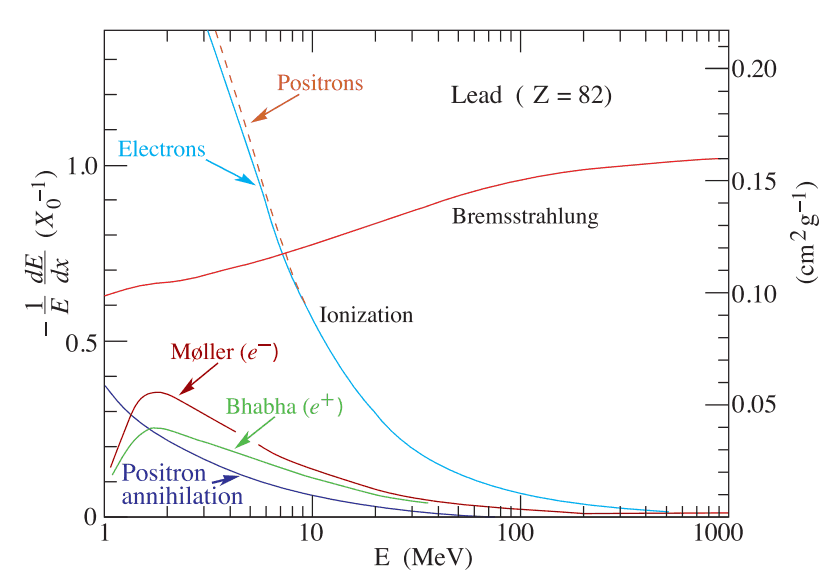
\includegraphics[width=.7\textwidth]{./img/electroninteractions.jpg}
	\caption{Energieverlust vs. Energie von verschiedenen Prozessen}
	\label{fig:electroninteractions}
\end{figure}
Elektronen können, je nach ihrer Energie, auf verschiedene Weisen mit Materie wechselwirken.
Dazu gehören die Prozesse
\begin{itemize}
	\item Möller-Streuung (einfach nur e an e)
	\item Bhabha-Streuung (einfach nur e an pos)
	\item Paarvernichtung und
	\item Bremsstrahlung
	\item Cherenkovstrahlung.
\end{itemize}
\autoref{fig:electroninteractions} zeigt den Energieverlust für verschiedene Energien und Prozesse.
Bremsstrahlung ist für hohe Energien dominant, Streuung und Ionisation für niedrige Energien.
Die \textbf{kritische Energie} ist dabei der Punkt, ab dem die Verluste durch Ionisation und Strahlung gleich sind.
Die Strahlungslänge $X_0$ ist definiert über
\begin{equation*}
	-\diff[E]{X} = \frac{E}{X_0}.
\end{equation*}

\subsection{Energieverlust durch Ionisation}
Die wichtigste Wechselwirkung geladener Teilchen ist die Ionisation des aktiven Mediums.
Dabei führt das Teilchen elastische Stöße mit den gebundenen Elektronen in den Atomen des Mediums aus.
Dies führt zu einem charakteristischen Energieverlust nach der \textbf{Bethe-Formel}
\begin{equation*}
	\diff[E]{X}\propto -z^2n_e\cdot\frac{1}{\beta^2}\log\left(\frac{2m_e\beta^2\gamma^2}{I} - \beta^2\right)
\end{equation*}
mit der Ladungszahl des Teilchens $z$, der Elektronendichte $n_e$ und der Ionisationsenergie $I$, welche mediumspezifisch ist.

Es fällt auf, dass die Ionisationsverluste unabhängig von der Masse des Teilchens sind.

Die Bethe-Formel beschreibt allerdings nur den mittleren Energieverlust.
Insbesondere in dünnen Absorbern führt dies zu von Fall zu Fall asymmetrischen Verteilungen.
Diese Fluktuationen werden empirisch durch die \textbf{Landau-Verteilung} beschrieben.

\subsection{Energieverlust durch Bremsstrahlung}
\begin{figure}
	\centering
	\begin{subfigure}{0.4\textwidth}
		\centering
		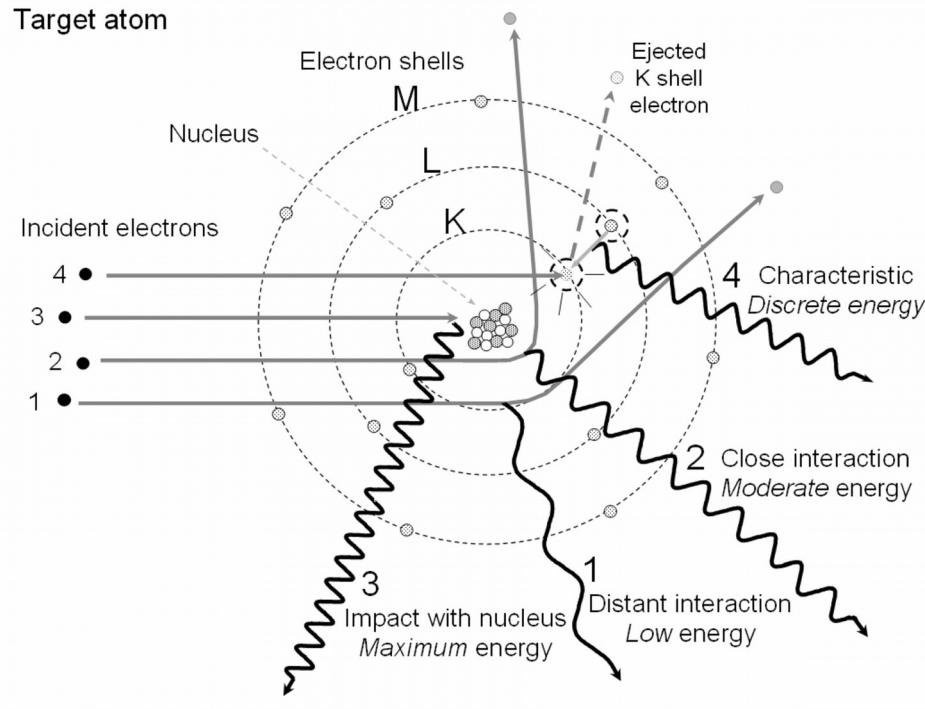
\includegraphics[width=\textwidth]{./img/elatom.jpg}
		\caption{Der Prozess der Bremsstrahlung}
		\label{fig:elatom}
	\end{subfigure}
	\begin{subfigure}{0.4\textwidth}
		\centering
		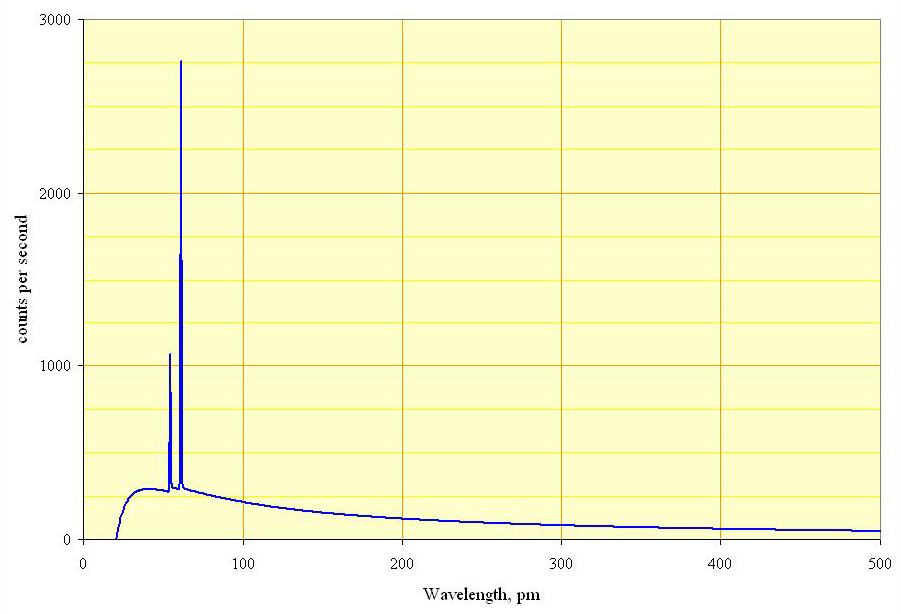
\includegraphics[width=\textwidth]{./img/bremsspec.jpg}
		\caption{Bremsstrahlungsspektrum mit überlagerten Floureszenzpeaks}
		\label{fig:bremsspec}
	\end{subfigure}
\end{figure}
Wird ein geladenes Teilchen beschleunigt, so emittiert es Bremsstrahlung.
Dabei ist die totale Strahlungsleistung für eine geradlinige Bewegung und eine Beschleunigung parallel zur Geschwindigkeit
\begin{equation*}
	P_\parallel = \frac{q^2a^2\gamma^6}{6\pi\varepsilon_0c^3}.
\end{equation*}
Wird das Teilchen allerdings orthogonal zu seiner Bewegungsrichtung beschleunigt (Kreisbahn), so ist
\begin{equation*}
	P_\perp = \frac{q^2a^2\gamma^4}{6\pi\varepsilon_0c^3}.
\end{equation*}
Da $\gamma = \frac{E}{mc^2}$ ist der Verlust durch Bremsstrahlung für schwere Teilchen deutlich geringer als für leichte.
Daher kann ein Elektronbeschleuniger im \si{\TeV}-Bereich aufgrund der geringen Elektronmasse niemals als Ringbeschleuniger realisiert werden, sondern nur als Linearbeschleuniger.

\autoref{fig:elatom} veranschaulicht den Prozess. In \autoref{fig:bremsspec} ist das daraus resultierende Spektrum zu sehen.
Das Bremsstrahlungsspektrum ist kontinuierlich, die Peaks im Spektrum sind Floureszenzen der Atome des Mediums.

\subsection{Cherenkovstrahlung}
Bewegt sich ein Elektron in einem unendlich weit ausgedehnten Medium ohne innere Struktur schneller als die Lichtgeschwindigkeit in diesem Medium, so wird Cherenkovstrahlung emittiert.
Dieses Phänomen lässt sich mit dem akustischen Phänomen des Überschallknalls vergleichen und ist das optische Analogon dazu.

Cherenkovstrahlung tritt nur unter einem festen Winkel unter der Bedingung
\begin{equation*}
	\cos\theta_\text{c} = \frac{1}{\beta n},
\end{equation*}
mit dem Brechungsindex $n$ des Mediums.

Man kann die Cherenkovstrahlung dazu verwenden, hochenergetische Teilchen zu detektieren.
So dient sie in einem Kernreaktor dazu, die augenblickliche Radioaktivität der Zerfallsprodukte zu bestimmen und ist somit ein Maß für die Reaktorleistung.

\section{Photonen}
Photonen können auf verschiedene Weisen mit Materie wechselwirken, dazu gehört
\begin{itemize}
	\item der Photoeffekt,
	\item die Compton-Streuung und
	\item die Paarbildung ($\el\pos$).
\end{itemize}

\subsection{Der Photoeffekt}
Als Photoeffekt bezeichnet man das Herauslösen von Elektronen aus dem Leitungs- bzw. Valenzband eines Atoms einer Halbleiter- oder einer Metalloberfläche durch ein anregendes Photon.
Der Wirkungsquerschnitt für diesen Prozess ist
\begin{equation*}
	\sigma = \frac{8\pi}{3}r_e^2Z^5\alpha^4\left(\frac{E_\gamma}{m_ec^2}\right)^\delta,
\end{equation*}
dabei ist $\delta$ von der Photonenenergie abhängig und nimmt verschiedene Werte an.
Auffällig ist die starke Abhängigkeit von der Kernladungszahl des Atoms, was Sinn ergibt, weil für große Kernladungszahlen die Coulomb-Abstoßung im Kern groß wird und daher nach der Bethe-Weizäcker-Formel (Coulombterm) das Atom weniger Bindungsenergie aufweist.
Daher ist für große Kernladungszahlen der Wirkungsquerschnitt auch entsprechend hoch.

	\chapter{Detektoren in der Teilchenphysik}
Was wir wissen wollen:
\begin{itemize}
	\item Transversalimpuls $p_\text{T}$
	\item Polarwinkel $\phi$
	\item (Pseudo)rapidität (also Azimuthwinkel) $\eta$
	\item Energie
	\item Teilchenart.
\end{itemize}

\section{Die Blasenkammer}
Das Prinzip der Blasenkammer ist einfach:
Die Flüssigkeit (z.B. H2) im Unterdruck beginnt an Verunreinigungen und Ionisationskeimen zu sieden.
Diese Bläschen werden fotografiert.
Das ist zum einen sehr ungenau und zum anderen können wir so keine Aussagen über die Teilchenart machen.

\section{Nachweismethoden für Teilchen}
\begin{figure}
	\centering
	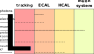
\includegraphics[width=.7\textwidth]{./img/detectorsystem.pdf}
	\caption{Verschiedene Teilchen können durch die Ebenen unterschieden werden.}
	\label{fig:detectionmethods}
\end{figure}
Um verschiedene Teilchenarten zu unterscheiden, ist ein Detektor durch mehrere Ebenen aufgebaut (siehe \autoref{fig:detectionmethods}).

\textbf{Die tracking layer} sorgt für eine Richtungsbestimmung.

\textbf{Das elektromagnetische Kalorimeter} bestimmt die Energie von Teilchen die im Wesentlichen über die elektromagnetische Kraft wechselwirken.

\textbf{Im hadronischen Kalorimeter} lassen sich Teilchen nachweisen, die überwiegend der starken Wechselwirkung unterliegen.
Da hadronische Teilchen szintillierendes Material fast ungehindert durchdringen ist der Nachweis über das em-Kalorimeter nicht gewährleistet.

\textbf{Im Myon-System} werden die hochenergetischen Myonen nachgewiesen, da sie für einen Nachweis im em-Kalorimeter zu hochenergetisch sind.

\section{Spurdetektoren}
\subsection{Gasgefüllte Spurdetektoren}
Hereinkommende geladene Teilchen ionisieren das Gas im Detektor und hinterlassen dabei eine Spur.
Ionisierte Ladungen bewegen sich entlang eines elektrischen Feldes zur Kathode bzw. Anode.
Je nach dem, in welchem Bereich der Kennlinie man sich bewegt unterscheidet man zwischen
\begin{itemize}
	\item \textbf{Proportionalkammern}, die im linearen Bereich der Kennlinie betrieben werden. Dabei ist die Anzahl der Ionenpaare proportional zur Primärionisation.
	\item \textbf{Geiger-Müller-Zählrohren}, die in der Plateauregion betrieben werden und damit keine Proportionalität zur Primärionisation aufweisen.
\end{itemize}
\subsubsection{Vieldrahtproportionalkammern}
bestehen aus vielen parallel angeordneten Anodendrähten. Es lässt sich somit eine 1D-Ortsinformation bestimmen und da sie im Proportionalbetrieb sind, auch die Teilchenenergie in einem bestimmten Bereich.

\subsubsection{Driftkammern}
lösen das Problem der limitierten Ortsauflösung durch den Drahtabstand bei MWPCs. Die Ionen brauchen eine bestimmte Zeit, um zum Anodendraht zu wandern. Diese Zeit $\Delta t$ kann dazu verwenden werden, um eine Ortsinformation zu erhalten nach
\begin{equation*}
	x' = x_0 + \frac{e}{2m}\mvec{E}(\mvec{r})\Delta t.
\end{equation*}
In Zeitprojektionskammern kann man so sogar eine 3D-Ortsbestimmung machen: 2D über die Projektion auf die Anoden, 1D über die Driftzeitinformation.

\subsection{Siliziumdetektoren}
Eleganter, aber kostenaufwändiger lässt sich das mit Siliziumdetektoren in Sperrrichtung lösen, wie am CMS der Fall.
Dabei beträgt die Impulsauflösung ca. 0.5\%.
Die Impulsbestimmung folgt aus dem assoziierten Zyklotronradius der Teilchenspur über
\begin{equation*}
	p[\si{\GeV}] = 0.3\cdot r[\si{\meter}] \cdot B[\si{\tesla}].
\end{equation*}

\section{Kalorimeter}
Das Kalorimeter schließt sich an die Spurdetektoren an und misst die Energie aller erzeugten und nachweisbaren Teilchen.
Dabei werden verschiedene Phänomene ausgenutzt
\begin{itemize}
	\item Energieverlust durch Ionisation
	\item Sammlung von Szintillationslicht
	\item Elektromagnetische und hadronische Schauerbildung.
\end{itemize}
Das Kalorimeter muss dabei dick genug sein, um die Teilchenschauer vollständig im aktiven Material zu stoppen, andernfalls gehen Informationen verloren.
Das Szintillationslicht wird dann durch Photomultiplier ausgelesen.
\subsection{Elektromagnetische Schauer}

\subsection{Hadronische Schauer}

\section{Das Myon-System}


	\chapter{Atome}

\section{Der Photoeffekt}
Bestrahlt man die Oberfläche eines Metalles mit Photonen, so werden Elektronen aus dieser herausgelöst.
Im Rahmen der klassischen Physik erscheinen bei diesem Versuch folgende Resultate als verwunderlich:
\begin{itemize}
	\item Die kinetische Energie der herausgelösten Elektronen hängt nicht von der Bestrahlungsstärke des Lichtes ab, sondern alleine von dessen Wellenlänge.
	\item Die kinetische Energie der Photoelektronen steigt ab einer Grenzfrequenz linear mit der Frequenz des Lichtes an.
	\item Die Grenzfrequenz hängt dabei nur vom Material der Kathodenoberfläche ab (Austrittsarbeit)
	\item Die Freisetzung der Elektronen beginnt instantan mit dem Einfall des Lichtes und endet genauso schnell auch mit dem Ende der Bestrahlung.
\end{itemize}

Man führt diese Beobachtungen auf den Teilchencharakter des Lichtes zurück.
Die Quantenmechanik konnte dabei erst den Welle-Teilchen-Dualismus des Lichtes deuten.

\section{Der Franck-Hertz-Versuch}
\begin{figure}
	\centering
	\begin{subfigure}{0.4\textwidth}
		\centering
		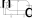
\includegraphics[width=\textwidth]{./img/fhversuch.pdf}
		\caption{Der Versuchsaufbau}
		\label{fig:fhversuch}
	\end{subfigure}
	\begin{subfigure}{0.4\textwidth}
		\centering
		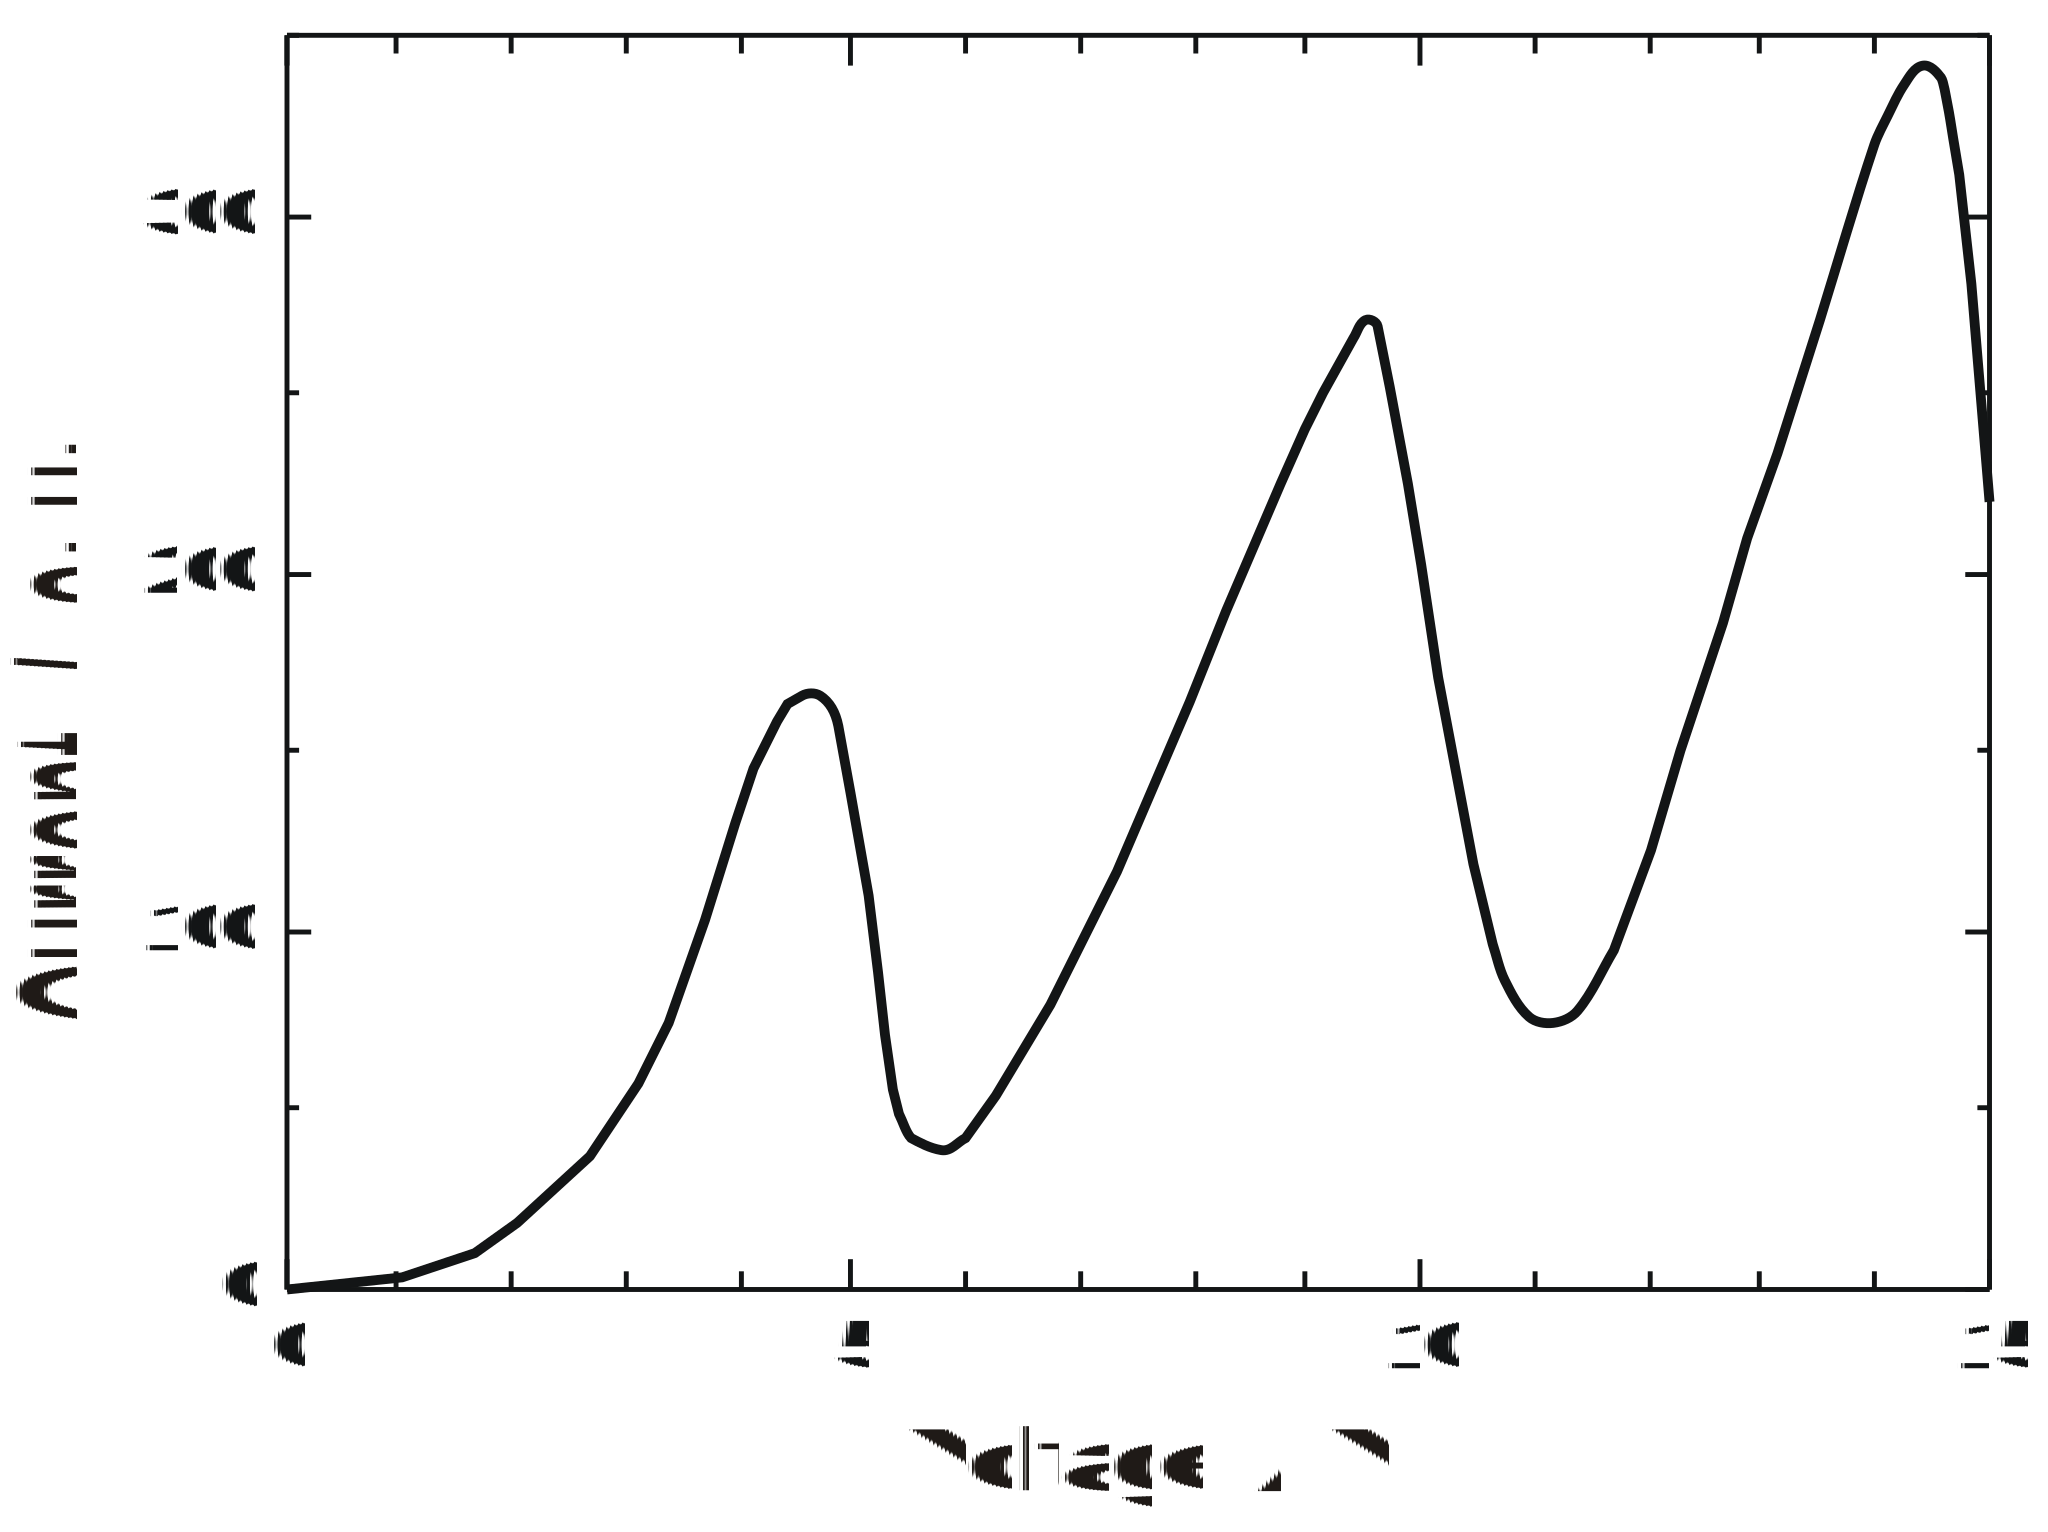
\includegraphics[width=\textwidth]{./img/fhspec.pdf}
		\caption{Der Anodenstrom in Abhängigkeit der Beschleunigungsspannung}
		\label{fig:fhspec}
	\end{subfigure}
	\caption{Der Franck-Hertz-Versuch}
\end{figure}
\textbf{Aufbau:}  \autoref{fig:fhversuch} zeigt den Aufbau des Versuches.
Im Glaskolben ist ein schwach unter Druck gesetztes Gas und 3 Elektroden.
Das Gitter ist gemeinsame Masse im Experiment.
Die Kathode $K$ wird auf negatives Potenzial gelegt und es werden durch diese Beschleunigungsspannung $U_\text{b}$ Elektronen aus der Kathode herausgelöst und zum Gitter hin beschleunigt.
Die meisten Elektronen landen dabei im Gitter und werden über die Spannungsquelle zur Kathode rückgeführt.
Einige Elektronen jedoch passieren das Gitter und fliegen dabei zur Auffangelektrode $A$.
$A$ wird dabei über die Gegenfeldspannung $U_\text{g}$ negativ aufgeladen und bremst somit die einfallenden Elektronen ab.
Die Spannung $U_\text{g}$ wird so weit erhöht bis gerade keine Elektronen mehr über das empfindliche Amperemeter messbar sind.

\textbf{Beobachtung}  Erhöht man $U_\text{b}$ bei festem $U_\text{g}$ und misst den Anodenstrom, so ergibt sich \autoref{fig:fhspec}.
Ab einem gewissen Wert sinkt der Anodenstrom ab und das wiederholt sich in (näherungsweise) festen Abständen.
Nach jeder Kante steigt dabei die Stromstärke auf einen höheren Wert.

\textbf{Erklärung}  Siehe \url{https://de.wikipedia.org/wiki/Franck-Hertz-Versuch#Erkl%C3%A4rung}.

\section{Die Planckverteilung}
Im Rahmen der klassischen Physik kann man die spektrale Leistungsverteilung eines schwarzen Körpers relativ einfach zu
\begin{equation*}
	M(\lambda)\cdot\text{d}\lambda = \frac{2\pi\cdot c\cdot k_\text{B}T}{\lambda^4}\cdot\text{d}\lambda.
\end{equation*}
Richtig ist dieses Verhalten bei großen Wellenlängen.
Jedoch strebt die Strahlungsleistung für kleine Wellenlängen gegen unendlich, was man als \textit{Ultraviolett-Katastrophe} bezeichnet.

Planck löste dieses Problem durch die Annahme, dass sich Wellen in einem Hohlraum (schwarzer Körper) sich verhalten wie harmonische Oszillatoren, die nur diskrete Energiewerte $E=n\cdot\hbar\omega$ annehmen können und bei diesen Energien Strahlung absorbieren/emittieren.
Einstein konnte die Planksche Strahlungsformel dann relativ einfach durch Mastergleichungen für das System (?) herleiten.
Die Übergänge lauteten
\begin{itemize}
	\item \textbf{Induzierte Emission:} $\text{d}N_{21} = B_{21}u(\nu)N_2\text{d}t$
	\item \textbf{Spontane Emission:} $\text{d}N_{21} = A_{21}N_2\text{d}t$.
\end{itemize}
Im thermischen Gleichgewicht folgt dann $\text{d}N_{21} = \text{d}N_{12}$ oder
\begin{equation*}
	\frac{N_2}{N_1} = \frac{B_{12}u(\nu)}{A_{21}+B_{21}u(\nu)} \stackrel{\text{Boltzm.}}{=} \frac{\exp(-E_1)}{\exp(-E_2)}.
\end{equation*}
Mit den Randbedingungen $T\rightarrow\infty : u(\nu)\rightarrow\infty$ und dass bei kleinen Frequenzen das Rayleigh-Jeans-Gesetz gelten muss, folgt dann die \textbf{spektrale Energiedichte der Photonen}
\begin{equation*}
	u(\nu) = \frac{8\pi h\nu^3}{c^3}\frac{1}{e^{\frac{h\nu}{k_\text{B}T}} - 1}.
\end{equation*}

Differenziert man diese Verteilung, ergibt sich das \textbf{Wien'sche Verschiebungsgesetz}
\begin{equation*}
	\lambda_\text{max}\cdot T = \text{const} = \SI{2.9e-3}{\kelvin\meter}.
\end{equation*}
Dieses Gesetz beschreibt die Lage des Peaks in der spektralen Leistungsverteilung der Strahlung eines Körpers.

\section{Das H-Atom}
Ohne relativistische Korrekturen, Fein-/Hyperfreinstruktur kann man die Schrödingergleichung für das Wasserstoffatom
\begin{equation*}
	\left(\frac{\hbar^2}{2m}-V_\text{c}(r)\right)\psi(r,\theta,\varphi) = E\psi(r,\theta,\varphi)
\end{equation*}
mit $V_\text{c}(r)=-\frac{e^2}{4\pi\varepsilon_0r}$ durch einen Separationsansatz
\begin{equation*}
	\psi(r,\theta,\varphi) = R_{nl}(r)\cdot Y_{lm}(\theta,\varphi)
\end{equation*}
lösen.
Dabei sind die $R_{nl}(r)$ im Wesentlichen die zugeordneten Laguerre-Polynome und $Y_{lm}(\theta,\varphi)$ die Kugelflächenfunktionen.
Diese Lösung führt auf die unkorrigierten Eigenenergien
\begin{equation*}
	E_n = -\frac{E_\text{R}}{n^2},
\end{equation*}
also ist das System hochgradig entartet bezüglich $l,m$.
$E_\text{R}$ ist die Rydberg-Energie, Wert irrelevant.

Die Energieniveaus spalten auf, wenn man die Fein-/Hyperfreinstruktur miteinbezieht.

\section{Stern-Gerlach-Experiment}
\textbf{Anordnung}  Ein Strahl von Silberatomen durchfliegt im Vakuum den Spalt zwischen den Polschuhen eines Magneten.
Durch die spezielle Form des Magneten weist das B-Feld quer zum Strahl eine starke Inhomogenität auf.
Nachdem der Strahl das Feld durchlaufen hat, schlagen sich die Silberatome auf einer Glasplatte nieder.

\textbf{Resultat}  Es werden zwei voneinander getrennte Flecke gefunden, das heißt, das Magnetfeld spaltet den Strahl in zwei getrennte Strahlen auf.

\textbf{Erklärung}  Da sich im Silberatom in der äußersten Valenzschale (5s) ein einzelnes Elektron befindet und sich der Gesamtdrehimpuls der inneren Schalen zu 0 addiert (abgeschlossene Schalen), besteht der Gesamtdrehimpuls der Atome also nur aus dem Spin dieses einen Elektrons.
Der entscheidende Unterschied zum Elektron ist hierbei aber, dass das Silberatom elektrisch neutral ist, somit im Magnetfeld keine Lorentzkraft erfahren kann.
Ferner könnte es auch nicht durch elektrische Störfelder abgelenkt werden.

Das Silberatom hat also ein magnetisches Dipolmoment $\mvec{\mu}$, auf das im inhomogenen Feld $\mvec{B}$ eine Kraft wirkt.
Klassisch müsste sich also, je nach Anstellwinkel zur Feldrichtung, eine kontinuierliche Aufweitung des Strahles in $\pm z$-Richtung beobachten lassen.

Da aber das magnetische Dipolmoment vom Drehimpuls $\mvec{S}$ her rührt und der Spin des Elektrons sich im Feld entweder parallel oder antiparallel anordnet (Quantenzahl $m=\pm\frac{1}{2}$), beobachtet man zwei diskrete Flecken.

Je nach dem, in welchem Orbital sich ein Valenzelektron befinden würde (s,p,d,f,\dots), würde man eine Aufspaltung in ggf. mehr als nur zwei Strahlen beobachten, je nach erlaubten Quantenzahlen $m$.

\section{Spin-Bahn-Kopplung und der Paschen-Back-Effekt}
Die Spin-Bahn-Kopplung ist in einem semiklassischen Modell eine Art ''interner Zeeman-Effekt''.
Das Feld wird dabei durch die Bahnbewegung der Elektronen erzeugt (Biot-Savart-Gesetz).
Das magnetische Moment des Spins koppelt somit an den Bahndrehimpuls.
Wenn wir also diese Korrektur in den Hamiltonian miteinbeziehen wird die Entartung z.B. im H-Atom teilweise aufgehoben
\begin{equation*}
	E_{nls} \propto E_n + \Delta E_\text{LS}(j,l).
\end{equation*}
Gute Quantenzahlen sind nun $n, l, s, j, m_j$.
Die Quantenzahl $j$ nimmt dabei die Werte $\{l+s,\dots,|l-s|\}$ an.

Zustände werden nun mit der Nomenklatur $n^{2s+1}l_j$ bezeichnet.

Wird nun allerdings ein großes, externes Magnetfeld angelegt, entkoppeln $\mvec{L}$ und $\mvec{S}$ und präzedieren unabhängig um die Richtung des magnetischen Feldes.
$J$ ist somit keine Quantenzahl von Eigenzuständen mehr.
Da $\mvec{L}$ und $\mvec{S}$ nun unabhängig an das magnetische Feld koppeln, ergibt sich ein neues Spektrum, das meistens einfacher aussieht, da weniger Zustände aufspalten.

Man nennt dieses Phänomen \textbf{Paschen-Back-Effekt}.

\section{LS-Kopplung bei Mehrelektronensystemen}
\subsection{Mehr Elektronen}
Bei moderat vielen Elektronen (bis etwa Kohlenstoff) addieren die Einzelspins und Einzelbahndrehimpulse zu Gesamtspins/-drehimpulsen
\begin{equation*}
	\mvec{L} = \sum_i\mvec{L_i}\quad\mvec{S} = \sum_i\mvec{S_i}.
\end{equation*}
Diese Gesamtdrehimpulse koppeln dann zum Gesamtdrehimpuls
\begin{equation*}
	\mvec{J} = \mvec{L} + \mvec{S}.
\end{equation*}

\subsection{Sehr viele Elektronen, hohe Kernladungszahlen}
Bei hohen Kernladungszahlen wird die Spin-Bahn-Wechselwirkung groß, weil $V_\text{LS}\propto Z^4$.
Dann liegt eine jj-Kopplung vor, bei denen für jedes Elektron für sich Spin-Bahn-Kopplung gilt
\begin{equation*}
	\mvec{j_i} = \mvec{l_i} + \mvec{s_i},
\end{equation*}
welche dann zu einem Gesamtdrehimpuls koppeln
\begin{equation*}
 \mvec{J} = \sum_i\mvec{j_i}.
\end{equation*}

\section{Hyperfeinstruktur}
Wird nun noch die Wechselwirkung des Kernspins mit dem elektronischen Magnetfeld miteinbezogen, so ergibt sich die Hyperfeinstruktur.
Wir führen einen neuen Gesamtdrehimpuls $\mvec{F} = \mvec{J} + \mvec{I}$ ein, mit dem bereits bekannten $\mvec{J} = \mvec{L} + \mvec{S}$ und dem Kernspin $\mvec{I}$.
Wie bei der LS-Kopplung spalten die Feinstrukturzustände nun wieder auf.
Dabei kann die Quantenzahl $f$ die Werte $\{j+i,\dots,|j-i|\}$ annehmen.

\textbf{Beispiel}  Wasserstoff im Zustand $2P_\frac{3}{2}$: $f=2,1$.
Die H-Energieniveaus spalten also auf in mindestens 2 Niveaus.

\section{Lamb-Shift}
Der Lamb-Shift ist eine Erklärung dafür, warum z.B. der Zustand $2S_\frac{1}{2}$ und $2P_\frac{1}{2}$ im Wasserstoffatom unterschiedliche Energien haben, obwohl die Dirac-Theorie vorhersagt, dass diese Zustände die gleiche Energie haben müssten.
Es lässt sich im Rahmen der QED dadurch erklären, dass die elektrischen und magnetischen Perturbationen im QED-Vakuum das elektrische Feld am Ort des Kerns stören.
Das ist ein One-Loop-Effekt in der QED, bei der ein Photon vom Atom emittiert und gleich wieder absorbiert wird.
Diese Störungen induzieren ihrerseits eine Störung des Position des Elektrons, welches aufgrund dessen eine Zitterbewegung ausführt.
Diese Zitterbewegung führt je nach $l$ und $j$ zu einem Shift in der Energie.

\section{Magnetische Resonanz}
Für den Grenzfall starker Magnetfelder ergibt sich aus dem Zeeman-Effekt bekanntermaßen der Paschen-Back-Effekt.
Betrachtet man die Hyperfeinstruktur eines Atomes, so entkoppeln für große Magnetfelder also analog zur LS-Kopplung der Gesamtdrehimpuls $\mvec{J}$ und der Kernspin $\mvec{I}$.
Diese Vektoren präzedieren unabhängig voneinander um die Magnetfeldachse.

Für die Energieverschiebung gilt
\begin{equation*}
	\Delta E_\text{HFS} = g_\text{J}\mu_\text{B}m_\text{J}B_0 - g_\text{I}\mu_\text{K}m_\text{I}B_0 + a\cdot m_\text{I}m_\text{J}.
\end{equation*}

\subsection{NMR}
Man kann sich dieses Energiesplitting bei der \textbf{magnetischen Resonanz} zu Nutze machen.
Der Vorgang dabei ist
\begin{itemize}
	\item Das Ausrichten der Kernspins durch ein externes, statisches Magnetfeld $B_0$.
	\item Die Störung dieser Ausrichtung durch ein schwaches, magnetisches Wechselfeld $B_\sim$.
\end{itemize}
Um den Präzessionskegel weitestmöglich zu weiten und damit effektiv das NMR-Signal zu erhöhen, wird das Wechselfeld orthogonal zum statischen Feld gewählt.
Die Frequenz des Wechselfeldes muss dabei der Larmorfrequenz des Kernes entsprechen, um Energieübergänge zwischen den Zeeman-Levels zu ermöglichen.
Es erfolgt also nur dann eine magnetische Resonanz, wenn $h\nu = g_\text{I}\mu_\text{K}B_0=\omega_\text{L}$.

Das selbe Prinzip kann man bei paramagnetischen Stoffen (Atome mit ungepaarten Elektronenspins) benutzen, die Resonanzbedingung ist dann aber durch das Bohr-Magneton und den Landé-Faktor des Elektrons zu ersetzen:
\begin{equation*}
	h\nu = g_\text{S}\mu_\text{B}B_0.
\end{equation*}
\begin{figure}
	\centering
	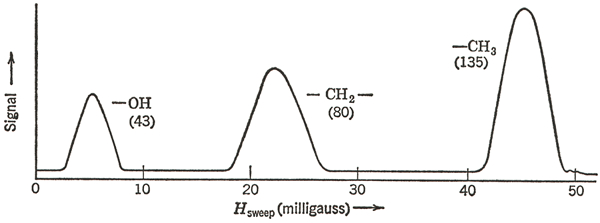
\includegraphics[width=.5\textwidth]{./img/nmrspec.jpg}
	\caption{NMR-Spektrum von Ethylalkohol. Die 3 Signale haben ein Flächenverhältnis 1:2:3. Sie gehören zu den Protonenspins in der Hydroxy-, Methylen- und Methylgruppe mit jeweils 1, 2, und 3 Protonen (H-Atome)}
	\label{fig:nmrspec}
\end{figure}
Man kann mit magnetischer Resonanz Spektroskopie betreiben.
In \autoref{fig:nmrspec} sieht man ein solches Spektrum, die Peaks sind Frequenzen des Wechselfeldes, für die die Resonanzbedingung erfüllt ist.
Da das Kernmagneton abhängig vom jeweiligen Kern ist, gibt es nach $h\nu = g_\text{I}\mu_\text{K}B_0$ verschiedene Frequenzen, für die das der Fall ist.

\section{Pauli-Prinzip: Ortho- und Parahelium}
Nach dem Pauli-Prinzip muss die Gesamtwellenfunktion von \textbf{Fermionen antisymmetrisch} und die von \textbf{Bosonen symmetrisch} unter Vertauschung zweier Teilchen sein.

Helium setzt sich aus 2 Elektronen und dem Kern zusammen.
Es gibt also zwei Möglichkeiten, eine antisymmetrische Wellenfunktion zu konstruieren:
\begin{itemize}
	\item \textbf{Parahelium:} Gesamtspin 0, d.h. antisymmetrische Spinwellenfunktion, symmetrische Bahnwellenfunktion.
	Beide Elektronen sind dabei im Grundzustand im 1s-Orbital. Singulett.
	\item \textbf{Orthohelium:} Gesamtspin 1, d.h. symmetrische Spinwellenfunktion, antisymmetrische Bahnwellenfunktion.
	Die Elektronen können demnach nicht im gleichen Orbital leben, im Grundzustand ist ein Elektron in 1s, das zweite in 2s. Triplett.
\end{itemize}

\section{Das Aufbauprinzip}
\begin{figure}
	\centering
	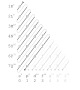
\includegraphics[width=.5\textwidth]{./img/madelung.pdf}
	\caption{Madelung-Schema zur Auffüllung der Schalen}
	\label{fig:madelung}
\end{figure}
Besetzt ein Elektron ein Orbital mit $l=n-1$, so haben wir es mit einem Orbital zu tun, das einer klassischen Kreisbahn sehr nahe kommt.
Für $l\ll n-1$ hingegen ist der Orbit stark elliptisch.
Das Elektron kommt auf seiner Tauchbahn dem unabgeschirmten Kern häufiger sehr nahe, was auf Grund der Attraktivität der Wechselwirkung zu einer Absenkung des Energieniveaus führt.
Schalen mit kleineren $(n+l)$-Werten werden aus diesem Grund vorher aufgefüllt.

\autoref{fig:madelung} zeigt das Madelung-Schema, mit dessen Hilfe die Reihenfolge der Auffüllung der Schalen klar wird.
Es gibt Ausnahmen dieses Aufbauprinzips bei einigen Elementen wie z.B. Lanthan, bei der zuerst die 5d-Unterschale besetzt wird, bevor die 4f-Schale aufgefüllt wird.
Diese Ausnahmen resultieren aus relativistischen Korrekturen und Elektron-Elektron-Korrelationen, die bei Atomen mit größeren Ordnungszahlen eine immer größere Rolle spielen.

\section{Hund'sche Regeln}
Um nun Auskunft über die Drehimpulskonfiguration der Elektronenhülle Auskunft geben zu können, werden die Hundschen Regeln eingesetzt, die prinzipiell nur für leichte Atome streng gelten, jedoch können auch für schwere Atome gute Ergebnisse erzielt werden.
Da die Literatur teilweise unverständlich erklärt, hier meine Version:
\begin{enumerate}
	\item Schau dir an, welche Schalen in dem zu bestimmenden Element nicht aufgefüllt sind.
	Die abgeschlossenen Schalen werden nach dem Aufbauprinzip einfach aufgefüllt und liefern nach dem Pauli-Prinzip einen Gesamtdrehimpuls 0.
	\item Die Spins innerhalb einer unaufgefüllten Schale wollen den Gesamtspin $S$ maximieren, daher orientieren sie sich möglichst parallel.
	Sobald jedoch die Schale zur Hälfte gefüllt ist, müssen nach dem Pauli-Prinzip die verbliebenen Spinplätze nun antiparallel aufgefüllt werden.
	Den Gesamtspin ergeben die ungepaarten Spins in der Schale, bei zwei ungepaarten z.B. $S=1$.
	\item Danach gilt: Gesamtbahndrehimpuls $L=\sum m_l$ muss maximal sein.
	Nach dem zweiten Schritt werden die Zustände ja zunächst mit ungepaarten Spins derselben Quantenzahl $m_s$ aufgefüllt, bis die Schale halb aufgefüllt ist.
	Dies bedeutet nach dem Pauli-Prinzip, dass alle $m_l$ von diesen Elektronen angenommen werden und daher der Gesamtbahndrehimpuls der halb aufgefüllten Schale $L=0$ ist.
	Als nächstes wird die andere Hälfte der Schale aufgefüllt. Um $L$ zu maximieren hat der erste gepaarte Spin dann $m_l=l$, der zweite $m_l=l-1$, usw.
	Das $L$ der teilweise aufgefüllten Schale wird also durch die gepaarten Spins bestimmt.
	\item Als Gesamtdrehimpuls $J$ ergibt sich dann:
	\begin{itemize}
		\item Schale weniger als halbvoll: $J=|L-S|$.
		\item Schale mehr als halbvoll: $J=L+S$.
	\end{itemize}
\end{enumerate}
Für ein Beispiel, siehe \url{https://de.wikipedia.org/wiki/Hundsche_Regeln#Anwendung}.

\section{Auger-Elektronen}
Nicht jeder atomare Übergang eines Elektrons führt zu einem emittierten Photon (Floureszenz).
Man nennt solche Übergänge \textbf{strahlungslose Übergänge}.

Ionisiert man durch externe Anregung ein Elektron auf einer der innersten Schalen (Beschuss mit Elektronen zum Beispiel), so füllt ein Elektron aus der nächsthöheren Schale das Loch auf.
Dabei relaxiert das Atom unter Emission eines Photons charakteristischer Frequenz.
Diesmal jedoch, wird dieses Photon direkt wieder in einer Schale des Atoms eingefangen und ionisiert ein Elektron einer höheren Schale, welches als sogenanntes \textbf{Auger-Elektron} emittiert wird.
Somit findet eine Relaxation ohne messbare Emission eines Photons statt.

	\chapter{Moleküle}
Das einfachste Molekül H2 lässt sich mit dem Hamiltonian
\begin{align*}
	H &= -\frac{\hbar^2}{2m}\laplacian_{\mvec{r_1}} -\frac{\hbar^2}{2m}\laplacian_{\mvec{r_2}} -\frac{\hbar^2}{2M}\laplacian_{\mvec{R_1}} -\frac{\hbar^2}{2M}\laplacian_{\mvec{R_2}} \\
	&+ \frac{e^2}{4\pi\epsilon_0} \left(\frac{1}{|\mvec{r_1}-\mvec{r_2}|} + \frac{1}{|\mvec{R_1}-\mvec{R_2}|} -\frac{1}{|\mvec{R_1}-\mvec{r_1}|} - \frac{1}{|\mvec{R_1}-\mvec{r_2}|} - \frac{1}{|\mvec{R_2}-\mvec{r_1}|} - \frac{1}{|\mvec{R_2}-\mvec{r_2}|} \right)
\end{align*}
beschreiben.
Dieses Problem ist analytisch so nicht lösbar, schon gar nicht für kompliziertere Moleküle.

\section{Die Born-Oppenheimer-Näherung}
Bedenkt man allerdings, dass die Kerne viel schwerer als die Elektronen - demnach auch viel langsamer - sind, kann man folgenden Ansatz machen:
\begin{equation*}
	\mvec{R} =: \mvec{R_2}-\mvec{R_1} = \text{const}.
\end{equation*}
Das Molekül rotiert also nicht und wir halten in Gedanken $\mvec{R}$ fest.

Ein Näherungs-Hamiltonian besteht dann aus
\begin{equation*}
	H_\text{Kern} = -\frac{\hbar^2}{2M_r}\laplacian_{\mvec{R}} + V_\text{eff}(R).
\end{equation*}
Die elektronische Bindung des Moleküls gibt dann das $V_\text{eff}(R)$ vor.

\section{Bindungen}

\subsection{Die kovalente Bindung}
Entsteht durch Überlapp der Wellenfunktionen der einzelnen Atome.

\textbf{Beispiel: Wasserstoffmolekül}  Die Bindung zwischen zwei H-Atomen entsteht aus einem Gleichgewicht der Coulomb-Abstoßung der Kerne und der anziehenden Austauschwechselwirkung der Elektronen.
Das Symmetrisierungspostulat der QM schreibt nun eine Verschränkung der Wellenfunktionen
\begin{align*}
	\psi_\text{s/a} = \varPsi(\mvec{x_1})\varphi(\mvec{x_2}) \pm \varphi(\mvec{x_1})\varPsi(\mvec{x_2})
\end{align*}
vor.
Es existieren also zwei Zustände: der bindende (sym.) und der antibindende (antisym.) Zustand.

Beim bindenden Zustand haben die Elektronen aufgrund des additiven Überlapps der Wellenfunktionen die größte Aufenthaltswahrscheinlichkeit zwischen den Kernen des Moleküls und schirmen somit die Coulomb-Abstoßung der Kerne teilweise ab.
Beim antibindenden Zustand jedoch, weisen die Elektronen keine Aufenthaltswahrscheinlichkeit zwischen den Kernen auf und es kommt zur Abstoßung der Atome.

\subsection{Van-der-Waals-Wechselwirkungen}
Edelgasatome (z.B. He) besitzen bereits eine sehr stabile $\el$-Konfiguration, daher ist keine kovalente Bindung möglich.
Jedoch können polarisierbare Moleküle induzierte Dipol-Dipol-Wechselwirkungen ausführen.

Um diese Bindung zu beschreiben, wird oft ein phänomenlogisches \textbf{Lennard-Jones-Potenzial}
\begin{equation*}
	V_\text{eff}(R) = 4\varepsilon\left( -\left(\frac{\sigma}{R}\right)^6 + \left(\frac{\sigma}{R}\right)^{12}\right)
\end{equation*}
angesetzt.

\subsection{Ionische Bindung}
Betrachten wir nun die Bindung zweier verschiedener Atome, z.B. Na und Cl.
Gibt das Na ein $\el$ an das Cl ab, so weisen beide abgeschlossene Schalen auf (energieärmster Zustand) und es entstehen ein Na+ und Cl- Ion.
Diese ziehen sich aufgrund der Coulomb-WW an.

\section{Molekülschwingungen}
\begin{figure}
	\centering
	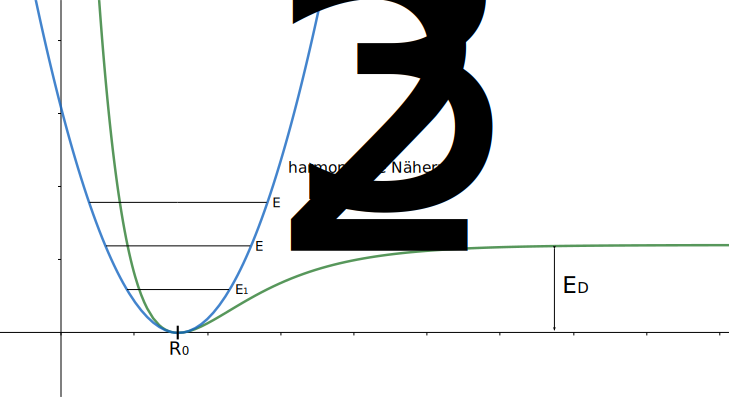
\includegraphics[width=.5\textwidth]{./img/harm_approx.pdf}
	\caption{Das \textsc{Morse}-Potenzial und die harmonische Näherung}
	\label{fig:harmapprox}
\end{figure}
Eine Molekülschwingung ist die periodische Bewegung von benachbarten Atomen innerhalb eines Moleküls.
Betrachten wir ein zweiatomiges Molekül, so wird das elektronische Potential in Abhängigkeit vom Kernbindungsabstand $R$ beschrieben durch das \textbf{Morse-Potenzial}
\begin{equation*}
	V_\text{M} = E_\text{D}\left(1 - e^{-a(R-R_0)}\right)^2.
\end{equation*}
Um das Problem leichter lösen zu können, machen wir (wie immer) eine harmonische Näherung
\begin{equation*}
	V_\text{M} \approx E_\text{D}a^2\left(R-R_0\right)^2.
\end{equation*}
Wie beim harmonischen Oszillator ergeben sich nun quantisierte Energieniveaus (siehe \autoref{fig:harmapprox}).
\begin{equation*}
	E_\nu = \hbar\Omega\left(\nu+\frac{1}{2}\right) - \frac{\hbar^2\Omega^2}{4E_\text{D}}\left(\nu+\frac{1}{2}\right)^2.
\end{equation*}
Atome können also zu Molekülschwingungen angeregt werden (z.B. durch Photonen).

\section{Molekülrotationen}

	\chapter{Kerne}

\section{Kernmodelle}
Die Masse eines Kernes ist
\begin{equation*}
	m_\text{Kern} = Z\cdot m_\text{p} + N\cdot m_\text{n} - E_\text{B}
\end{equation*}
mit $Z$, der Kernladungszahl, $N$, der Neutronenzahl und $E_\text{B}$, der Bindungsenergie.

Es gibt verschiedene Modelle, diese Bindungsenergie zu beschreiben.

\subsection{Tröpfchenmodell}
Das Tröpfchenmodell beschreibt einen Atomkern wie einen Flüssigkeitstropfen.
Die darauf beruhende \textbf{Bethe-Weizsäcker-Massenformel} lautet
\begin{equation*}
	E_\text{B} = \underbrace{a_\text{V}A}_{E_\text{V}} - \underbrace{a_\text{S}A^\frac{2}{3}}_{E_\text{S}} - \underbrace{a_\text{C}\frac{Z(Z-1)}{A^\frac{1}{3}}}_{E_\text{C}} - \underbrace{a_\text{A}\frac{(A-2Z)^2}{A}}_{E_\text{C}} + \delta (A,Z).
\end{equation*}

\subsubsection{Der Volumenterm $E_\text{V}$}
Der Volumenterm $E_\text{V}$ ist proportional zum Volumen $V$ des Kerns, welcher proportional zu $A$ ist.
Es liegt dabei die starke Wechselwirkung zugrunde, die bekanntlich gleichermaßen auf Protonen und Neutronen wirkt, daher überrascht es nicht, dass kein $Z$ im Term vorkommt.
Die Zahl der möglichen Wechselwirkungspaare ist $\frac{A(A-1)}{2}$, also würde man naiv einen Term erwarten, der wie $A^2$ geht.
Allerdings hat die starke Wechselwirkung nur eine sehr begrenzte Reichweite, sodass nur nächste und übernächste Nachbarn wechselwirken können, daher geht der Term etwa linear in $A$.

\subsubsection{Der Oberflächenterm $E_\text{S}$}
Der Oberflächenterm $E_\text{S}$ basiert ebenfalls auf der starken Wechselwirkung.
Er ist eine Korrektur zum Volumenterm für Teilchen am Rand des Tropfens, der beachtet, dass Nukleonen an der Oberfläche des Tropfens weniger Wechselwirkungspartner zur Verfügung haben.
Wenn also das Volumen des Tropfens $\propto A$ ist, dann ist die Oberfläche $\propto A^\frac{2}{3}$, daher die Form.
Das Analogon zum Tropfen ist hier die Oberflächenspannung.

\subsubsection{Der Coulombterm $E_\text{C}$}
Dem Coulombterm $E_\text{C}$ liegt die elektrostatische Abstoßung zwischen den Protonen zugrunde.
Da die Abstoßung nur für mehr als ein Proton existieren kann, folgt die Form $Z(Z-1)$.
Wenn man annimmt, dass der Tropfen eine gleichmäßige Ladungsverteilung hat, so geht das elektrische Feld mit $\frac{1}{R}\propto\frac{1}{A^\frac{1}{3}}$.

\subsubsection{Der Asymmetrieterm $E_\text{A}$}
Beim Asymmetrieterm $E_\text{A}$ kommt das Pauli-Prinzip zum Tragen.
Sowohl Protonen, als auch Neutronen können unter Beachtung des Pauli-Prinzips innerhalb ihrer eigenen Pools Energieniveaus bis zu ihrer Fermienergie auffüllen.
Wenn nun von einer Sorte Nukleonen mehr Teilchen im Kern vorhanden sind, so hat dieser Pool eine höhere Fermienergie als der andere.
Wir könnten durch einen schwachen Zerfall nun die Energie senken, daher ist die Energie höher, als sie sein müsste.
Diese Überlegung bildet die Basis dieses Termes.

Im Fermigasmodell für Kerne folgt dieser Term sogar explizit aus der Rechnung.

\subsubsection{Der Paarungsterm $\delta$}
Dieser Term erfasst den Effekt der Spinkopplung und ist gegeben durch
\begin{equation*}
	\delta(A,Z) = \begin{cases}
									+\delta_0\quad\text{gg-Kerne} \\
									0 \quad\text{ug-Kerne} \\
									-\delta_0\quad\text{uu-Kerne} \\
								\end{cases}
\end{equation*}

\subsection{Das Fermigasmodell}
Im Fermigasmodell der Kerne betrachtet man die Neutronen und Protonen innerhalb des Kernes als (wechselwirkungsfreie), ideale Fermi-Gase bei $T=0$.
Gemäß den Lehren der statistischen Physik kann man somit die Fermienergie der Gase herleiten
\begin{equation*}
	\varepsilon_\text{n/p} = \left(\frac{9\pi}{4}\right)^\frac{2}{3} \frac{\hbar^2}{2m_\text{n/p}R_\text{s}^2}\left(\frac{\{N/Z\}}{A}\right)^\frac{2}{3}.
\end{equation*}

Der Asymmetrieterm im Tröpfchenmodell findet seine Begründung im Fermigas-Modell, wie bereits erläutert.
Man kann mit dem Fermigasmodell gut die Größenordnungen der Energien abschätzen, jedoch ist der Gültigkeitsbereich des Modells sehr beschränkt.
In einem nächsten Schritt könnte man die Wechselwirkung der Gase miteinbeziehen, was zu einer Korrektur führen würde.

\subsection{Schalenmodell}
Ein weiteres, sehr erfolgreiches Modell zur Beschreibung der Kerne ist das Schalenmodell.

\subsubsection{Magische Zahlen}
Experimentell beobachtet man, dass Kerne mit bestimmten Protonen- bzw. Neutronenzahlen besonders stabil sind.
Man nennt diese bestimmten Zahlen \textbf{magische Zahlen}.
Sie lauten
\begin{equation*}
	2, 8, 20, (28\text{, Neutronen}), 50, 82, 126 \dots
\end{equation*}
Außerordentlich stabil sind dabei \textbf{doppelt-magische} Kerne.
Diese Tatsache suggeriert Schalenabschlüsse, wie im Atommodell, allerdings gibt es hier den Unterschied, dass es kein dominierendes Zentralpotenzial gibt.

\subsubsection{Das Modell}
Man betrachtet die Zustände eines Nukleons in einem von den anderen Nukleonen erzeugten Feld.
Jeder Zustand ist dabei nach dem Pauli-Prinzip besetzt.

Setzt man ein radialsymmetrisches, im Inneren konstantes und scharfrandiges Potenzial an, so faktorisiert die Schrödingergleichung in einen Radial- und Winkelanteil.
Am besten scheint experimentell dabei ein Fermi-ähnliches Potenzial zu passen, das \textbf{Woods-Saxon-Potenzial}
\begin{equation*}
	V(r) = -\frac{V_0}{1+e^\frac{r-R}{a}}.
\end{equation*}
Leider ist dieses Potenzial analytisch nicht lösbar, weshalb man ein ähnlich verlaufendes, modifiziertes, harmonisches Potenzial verwendet.

Jedenfalls erhält man als Lösungen der Schrödingergleichung diskrete Energieniveaus, die je nach Quantenzahlen bestimmte Anzahlen an Teilchen aufnehmen können
\begin{equation}\label{eq:eniveaus}
	E_{n,l} = \hbar\omega\left(2(n-1) + l + \frac{3}{2}\right).
\end{equation}
Die ersten 3 magischen Zahlen können so durch die Auffüllung der Energieniveaus erklärt werden, jedoch ab der vierten nicht mehr.
Daher kann ein reines Zentralpotenzial nicht die Lösung sein.

Hier muss nun die Spin-Bahn-Kopplung der Nukleonen miteinbeziehen
\begin{equation*}
	\tilde{V}(r) = V_0(r) + V_{ls}(r)\frac{\mvec{l}\cdot\mvec{s}}{\hbar^2}.
\end{equation*}
\textbf{Nach \autoref{eq:eniveaus} ist $l$ allerdings nicht wie beim Atommodell nach oben durch $n$ beschränkt, sondern kann beliebige Werte annehmen!}
Daher ist die Spin-Bahn-Kopplung im Kern insbesondere für große $l$ sehr groß!

Mit diesem Modell können nun alle magischen Zahlen erklärt werden, da Niveaus mit größerem Gesamtdrehimpuls hier energetisch günstiger sind.
Atome wollen also den Gesamtdrehimpuls minimieren, während Kerne ihn maximieren wollen.

\section{Instabile Kerne}
Instabile Kerne können über verschiedene Zerfälle in stabile Kerne zerfallen.

\subsection{$\upgamma$-Strahlung}
Angeregte Kerne verlieren überschüssige Energie durch monoenergetische Photonenemission.
Da die elektromagnetische Wechselwirkung paritätserhaltend und drehimpulserhaltend ist, müssen sogenannte \textbf{Auswahlregeln} beachtet werden
\begin{equation*}
	|J_f-J_i|\leq l\leq J_f+ J_i\quad (0\rightarrow 0\ \text{aber verboten!}).
\end{equation*}

\subsection{$\upbeta$-Zerfall}
\begin{figure}
	\centering
	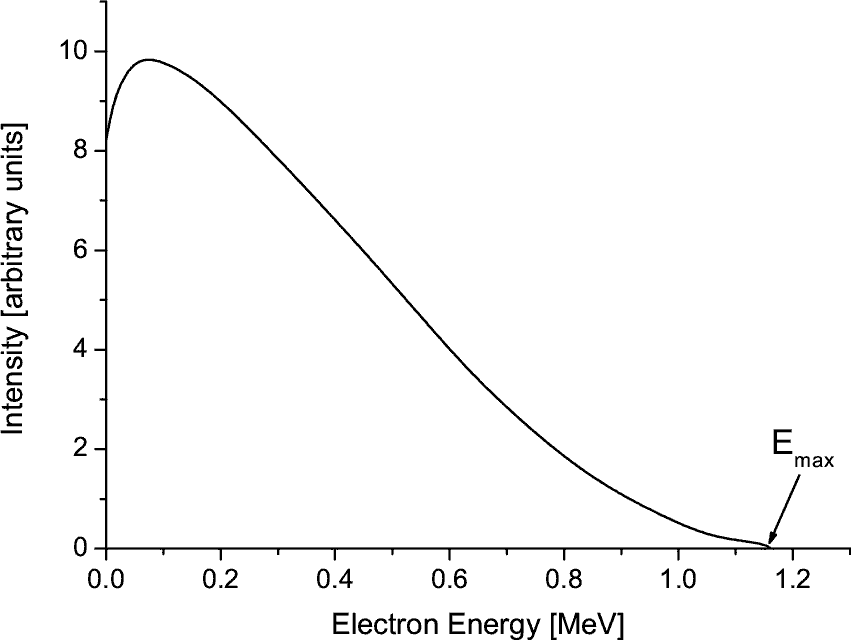
\includegraphics[width=.5\textwidth]{./img/betaspec.jpg}
	\caption{Elektronspektrum des Betazerflls von Bi-210}
	\label{fig:betaspec}
\end{figure}
Kerne können über die schwache Wechselwirkung einen $\upbeta$-Zerfall ausführen und zerfallen in ein Isotop der benachbarten Elemente.
Da der $\upbeta$-Zerfall ein 2-Körperzerfall ist, ist das Elektronspektrum kontinuierlich, da sich der Impuls auf das Neutrino und das Elektron verteilen kann, wie man in \autoref{fig:betaspec} sehen kann.

\subsection{$\upalpha$-Zerfall}
Kerne können sich auch über die Emission eines He-4 Kernes umwandeln.
Das dabei emittierte Alphateilchen ist monoenergetisch und die Energie hängt von der Energiebilanz (Bindungsenergien) und der Masse des Kernes ab.

\subsection{Anwendung: CNO-Zyklus}
\begin{figure}
	\centering
	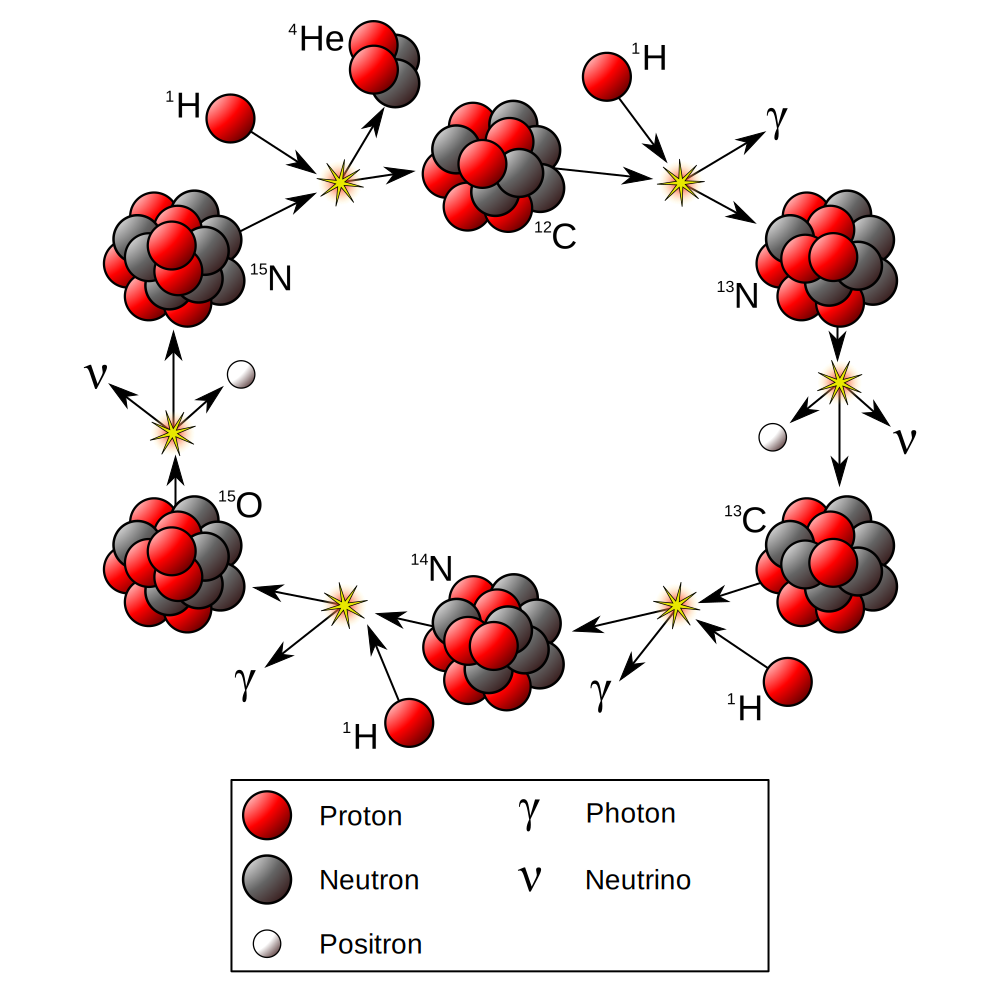
\includegraphics[width=.5\textwidth]{./img/cno.pdf}
	\caption{Der CNO-Zyklus}
	\label{fig:cno}
\end{figure}
Der CNO-Zyklus ist eine der acht Fusionsreaktionen des so genannten Wasserstoffbrennens, durch die Sterne Wasserstoff in Helium (und dann in schwerere Elemente) umwandeln.
Er ist in \autoref{fig:cno} abgebildet.

\subsection{Anwendung: Big-Bang-Nucleosynthesis}
Direkt nach dem Urknall war das Universum sehr dicht und sehr heiß.
Das Verhältnis von Protonen und Neutronen (aus dem Quark-Gluon-Plasma am Anfang) war im thermischen Gleichgewicht etwa 1:1, da die dominanten Übergänge
\begin{align*}
	n + \pos &\rightleftharpoons \bar{\nu_e} + p \\
	n + \nu_e &\rightleftharpoons p + \el
\end{align*}
aufgrund der hohen Temperatur und Dichte schnell abgelaufen sind.

Während der Abkühlung ($t<\SI{1}{\second}$) jedoch tendierte das Gleichgewicht immer mehr zu den Protonen, da diese eine etwas kleinere Masse als Neutronen haben.
Das Universum kühlte sich immer weiter ab und das Verhältnis \nicefrac{n}{p} sank immer weiter, bis die Temperatur und Dichte zu niedrig waren und damit die Reaktionen zu langsam abliefen.
Zu diesem Zeitpunkt war das Verhältnis bei etwa \nicefrac{1}{6}.
Da freie Neutronen instabil mit einer Halbwertszeit von $\SI{880}{\second}$ sind, zerfielen noch ein paar Neutronen bevor sie sich zu Kernen binden konnten
\begin{equation*}
	n \longrightarrow p + \el + \bar{\nu_e}.
\end{equation*}
Damit war das Verhältnis schlussendlich bei etwa \nicefrac{1}{7} angekommen.

Da He-4 die größte Bindungsenergie unter den leichten Elementen hat, verbanden sich die Neutronen überwiegend zu He-4-Kernen.

	\chapter{Festkörperphysik}

\section{Konstruktion der Wigner-Seitz-Zelle}
Einen Gitterpunkt wählen und Verbindungsstrecken zu sämtlichen anderen Gitterpunkten durch Normalebenen halbieren.
Eingegrenztes Gebiet ist dann Wigner-Seitz-Zelle.

\section{Das reziproke Gitter}
Das zu einem Ortsraumgitter reziproke Gitter ist definiert durch
\begin{equation*}
	\mvec{K} = h\mvec{A_1} + k\mvec{A_2} + l\mvec{A_3}\quad h,k,l\in\mathbb{Z}.
\end{equation*}
Dabei muss die Relation
\begin{equation*}
	\mvec{A_i}\mvec{a_j} = 2\pi\delta_{ij}
\end{equation*}
erfüllt sein.
Man kann die Vektoren $\mvec{A_i}$ durch die Konstruktionsvorschrift
\begin{equation*}
	\mvec{A_i} = 2\pi\varepsilon_{ijk}\frac{\mvec{a_k}\times\mvec{a_k}}{\mvec{a_1}\cdot(\mvec{a_2}\times\mvec{a_3})}.
\end{equation*}

\section{Beugung am Gitter}
Damit eine Beugung auftritt muss gelten
\begin{equation*}
	\Delta\mvec{k} = \mvec{K},
\end{equation*}
mit $\Delta\mvec{k}=\mvec{k}-\mvec{k'}$, dem Differenzwellenvektor der einfallenden Welle und $\mvec{K}$ einem reziproken Gittervektor.

Multiplizieren wir von links mit $\mvec{a_i}$, dann erhalten wir die \textbf{Laue-Bedingung}
\begin{align*}
	\mvec{a_1}\cdot\Delta\mvec{k} &= 2\pi h \\
	\mvec{a_2}\cdot\Delta\mvec{k} &= 2\pi k \\
	\mvec{a_3}\cdot\Delta\mvec{k} &= 2\pi l.
\end{align*}

Andere Form:
\begin{equation*}
	\mvec{G}^2 = 2\mvec{k}\cdot\mvec{G}.
\end{equation*}

Andere Form:
\begin{equation*}
	2d\sin\theta = m\lambda\quad m\in\mathbb{Z}.
\end{equation*}

\section{Die erste Brillouin-Zone}
Die erste Brillouin-Zone ist die Wigner-Seitz-Zelle des reziproken Gitters.
Nach der ersten Brillouin-Zone wiederholt sich die gesamte Kristallstruktur periodisch, d.h. es reicht, alle Prozesse in der ersten Brillouin-Zone zu beschreiben, um die Physik des Kristalles vollständig zu charakterisieren.

\section{Atomstrukturfaktoren}
Wie bereits aus der Streuung bekannt, ist die Streuamplitude in Bornscher Näherung die FT der Ladungsverteilung
\begin{equation*}
	f(\mvec{k})\propto\int_{-\infty}^\infty\text{d}^3r\rho(\mvec{r})e^{-i\Delta\mvec{k}\cdot\mvec{r}} = N\cdot\underbrace{\int_\text{EZ}\text{d}^3r\rho(\mvec{r})e^{-i\mvec{K}\cdot\mvec{r}}}_\text{Strukturfaktor}.
\end{equation*}
Befinden sich nun $s$ Atome in der Einheitszelle, so können wir den Strukturfaktor schreiben als
\begin{equation*}
	S_{\mvec{K}} = \sum_j^se^{-i\mvec{K}\cdot\mvec{r_j}}\underbrace{\int_\text{EZ}\text{d}^3r\rho(\mvec{r}-\mvec{r_j})e^{-i\mvec{K}\cdot(\mvec{r}-\mvec{r_j})}}_\text{Atomformfaktoren $f_j$}.
\end{equation*}
Ersetzen wir schlussendlich $\mvec{K}\cdot\mvec{r_j} = 2\pi(hx_{1j} + kx_{2j} + lx_{3j})$, so ergibt sich
\begin{equation*}
	S_{\mvec{K}}(h,k,l) = \sum_j^sf_je^{-2\pi\iu(hx_{1j} + kx_{2j} + lx_{3j})}.
\end{equation*}

Wir interpretieren:
Selbst wenn die Bragg-Bedingung für eine Beugung erfüllt ist, hängt es von der Basis ab, ob der Strukturfaktor 0 ist und somit kein Beugungsreflex sichtbar ist.

\textbf{Beispiel}  bcc, z.B. Metall-Na. Kubische Einheitszelle mit Basisatomen $\mvec{r_1} = (000)^\text{T}$ und $\mvec{r_2} = \frac{1}{2}(111)^\text{T}$.
\begin{equation*}
	S_{\mvec{K}}(h,k,l) = f\cdot\begin{cases}
																0,\quad(h+k+l)\text{ gerade} \\
																2,\quad(h+k+l)\text{ ungerade}
															\end{cases}
\end{equation*}
Also liefern in diesem Fall nur Miller-Ebenen mit $(h+k+l)$ ungerade einen Beugungsreflex.

\section{Der Debye-Waller-Faktor}
Betrachtet man endliche Temperaturen $T$, so sind die Gitteratome nicht stationär, sondern führen kleine Oszillationen aus.
Unter einer harmonischen Näherung dieser Oszillationen ergibt sich für die Intensität einer gestreuten Welle dann
\begin{equation*}
	I = I_0\cdot e^{-\frac{k_\text{B}T}{m\omega^2}\mvec{K}^2}.
\end{equation*}
Die Beugungsintensität nimmt also mit steigender Temperatur ab.

\section{Beugungsverfahren}
\subsection{Debye-Scherrer}
Röntgenstrahlen treffen auf kristallines Pulver, in dem die Kristalliten in zufälliger räumlicher Anordnung vorliegen.
Ein paar Kristalliten erfüllen mit ihrer Orientierung dabei die Bragg-Bedingung und werden gebeugt.
Aus den Durchmessern der Beugungsringe im Diffraktogramm lässt sich dann über die Bragg-Bedingung $2d\sin\theta = m\lambda$ Rückschluss auf den Netzebenenabstand $d$ und unter Miteinbeziehung der Millerschen Indizes dann auch die Gitterkonstanten ziehen.

\subsection{Laue}
Polychromatische Röntgenstrahlen treffen auf Einkristall.
Es sind Beugungspunktreflexe zu sehen.
Dadurch, dass die Röntgenstrahlen polychromatisch sind, erfüllen mehrere Gitterschichten die Bragg-Bedingung gleichzeitig.
Dadurch lässt sich aber ein bestimmter Reflex nicht mehr eindeutig einer Wellenlänge zuordnen.
Die Datenverarbeitung ist daher meist mühsam und zeitaufwändig.

\section{Phononen: Lineare Kette}
Betrachten wir nun eine lineare Kette aus miteinander gekoppelten Atomen (modelliert durch Kugeln der Massen $m(M)$ verbunden durch Federn mit Federkonstante $D\rightarrow$ harmonische Näherung).

Da das System eine diskrete Natur aufweist, ist die Zahl der unterscheidbaren Vibrationsmoden endlich, wobei $\lambda_\text{min}=2a$ und $\lambda_\text{max}=2L$ (mit der Kettenlänge $L$) die minimalen und maximalen Wellenlängen der Moden sind.
Definiert man nun eine \textbf{Modenzahl} $n=\frac{2L}{\lambda_n}$, folgt die maximale Zahl der Moden
\begin{equation*}
	n_\text{max}=\frac{2L}{\lambda_\text{min}}=\frac{L}{a},
\end{equation*}
welche gleich der Anzahl Atome in der Kette ist.

Auf gleiche Weise erhalten wir die maximale Wellenzahl
\begin{equation*}
	k_\text{max}=\frac{2\pi}{\lambda_\text{min}}=\frac{\pi}{a},
\end{equation*}
die mit den Grenzen der ersten Brillouin-Zone für ein einfach kubisches Gitter übereinstimmt.

\subsection{Gleiche Massen}
\begin{figure}[tbp]
	\centering
	\includegraphics[width=0.5\textwidth]{./img/dispersion_single.pdf}
	\caption{\textbf{Dispersionsrelation für identische Atome} Jede mögliche Frequenz taucht im Intervall zwischen 0 und $\frac{\pi}{a}$ auf, was bedeutet, dass jede Wellenzahl außerhalb dieser ersten Brillouin-Zone ununterscheidbar von einer bereits darin enthaltenen Schwingung ist.}
	\label{fig:dispersion_single}
\end{figure}
Sind nur Atome von der gleichen Sorte (Masse $m$) vorhanden, lässt sich durch Aufstellen der Newtonschen Bewegungsgleichung einfach die Dispersionsrelation
\begin{equation}
	\omega(k) = \sqrt{\frac{4D}{m}}\abs{\sin\left(\frac{ka}{2}\right)}
\end{equation}
herleiten, die in \autoref{fig:dispersion_single} aufgetragen ist.

Für kleine $k$ ist $\sin(k)\approx k$, daher folgt für die Dispersionsrelation
\begin{equation*}
	\omega(k)\approx \sqrt{\frac{Da^2}{m}}\abs{k}.
\end{equation*}
Es folgt also, dass für diesen Fall, die Phasen ($v_\text{ph}=\frac{\omega}{k}$)- und Gruppengeschwindigkeit ($v_\text{gr}=\frac{\text{d}\omega}{\text{d}k}$) gleich ist
\begin{equation}\label{eq:sound_single}
	v_\text{ph} = v_\text{g}\approx \sqrt{\frac{Da^2}{m}}.
\end{equation}

\subsection{Zwei Atomsorten}
\begin{figure}[tbp]
	\centering
	\includegraphics[width=0.5\textwidth]{./img/dispersion_alternating.pdf}
	\caption{\textbf{Dispersionsrelation einer Kette mit zwei Atomsorten (abwechselnd)} Zwischen dem optischen und akustischen Zweig der Dispersionsrelation ist eine \textbf{Bandlücke} sichtbar (rot). Wellen mit Frequenzen innerhalb dieser Lücke können im Kristall nicht propagieren.}
	\label{fig:dispersion_alternating}
\end{figure}
Enthält die Kette nun zwei verschiedene Atomsorten der Massen $m_1$ und $m_2$, so hat die Dispersionsrelation nach der Lösung der Bewegungsgleichungen zwei Lösungen:
\begin{equation}
	\omega_\pm^2(k) = \frac{D}{\mu} \pm D\sqrt{\frac{1}{\mu^2} - \frac{4}{m_1 m_2}\sin^2\left(k a\right)},
\end{equation}
mit der reduzierten Masse $\mu = \frac{m_1 m_2}{m_1 + m_2}$.

Für Kristalle mit mindestens zwei verschiedenen Atomsorten in einer primtiven Elementarzelle erzeugt die Dispersionsrelation zwei Arten von Photonen, die akustischen und optischen Phononen.
Sie korrespondieren jeweils mit den $\omega_{-}$ und $\omega_{+}$ Lösungen, welche in \autoref{fig:dispersion_alternating} zu sehen sind (+ ist opt., - ist akust.).
In akustischen Moden schwingen alle Atome in Phase, während bei optischen Moden jedes Nachbaratom einen Phasenversatz von 180° relativ zum nächsten hat.
Daher entsteht eine Bandlücke in einer bestimmten Frequenzgegend, sodass Wellen mit Frequenzen innerhalb dieser Bandlücke nicht propagieren können.

	%\include{bibliography.ag}
\end{document}
